\chapter{基于用户交互的ASP解释模型的设计}
针对现有ASP程序解释和调试难以同时满足规模适当与解释清晰完备的问题,本文试图将用户交互引入解释与调试之中。其中,基于用户交互的ASP程序解释模型是调试模型的基础,本章介绍这一模型,主要包括以下几方面内容,首先找到一种合适的ASP程序图表示方法,进一步面向ASP程序的解释对图中的环进行处理,提出ASP程序的解释空间及其构建算法,基于解释空间定义交互解释模型,讨论解释中的用户交互,最后针对非实例化程序的解释,讨论当前实例化工具面向解释存在的问题并给出适当的实例化方案。
\section{面向解释的ASP程序图表示}
面向人工智能可解释对易于人接受的要求,结合图对于关联关系直观表达的特性,本文设计基于文字-规则依赖图的方法对ASP程序的解释进行表示。因此,首先需要定义一种面向解释的ASP程序图表示法,该表示法应能够简洁、完整地说明程序中规则和文字之间的依赖关系。第\ref{chp:introsuction}章已有的研究中,已经提出了许多与ASP程序相关的图表示方法,包括依赖图(DG,Denpendency Graph)\cite{apt1994logic},规则图(RG,Rule Graph)\cite{dimopoulos1996graph}和扩展依赖图(EDG,Extended Dependency Graph)\cite{brignoli2014characterizing}。在交互解释的需求中,尽可能详细地保留与程序相关的所有文字和规则能够为用户提供更丰富、灵活的选择。而上述三种图表示中,只有EDG在表示中既包含程序中的规则又包含程序中的原子。因此,基于EDG的思想,本文定义了一种原子-规则图(ARG,Atom-Rule Graph),这种表示直观地呈现了原子与规则之间的依赖关系。

\begin{definition}[原子-规则图ARG]
    给定一个实例化的一致性ASP程序$P$,该程序的原子-规则图ARG(记为$ARG_P$)定义一张图$\langle V, E \rangle $,其中:
    \begin{itemize}[topsep=0pt]
      \setlength\itemsep{-0.3em}
      \item $V=V_{atom} \cup V_{rule} \cup V_{sink}$表示$ARG_P$中的所有结点组成的集合,其中:
      \begin{itemize}[label=$\circ$,topsep=0pt]
        \setlength\itemsep{-0.3em}
        \item $V_{atom} = At(P)$ 是$ARG_P$中所有的 \textbf{原子结点},表示$P$中出现的所有原子;
        \item $V_{atom} = R(P)$ 是$ARG_P$中所有的 \textbf{规则结点},表示$P$中出现的所有规则;
        \item $V_{sink} = \{Fact, NH\}$ 是图中唯一可能的两个汇点的集合,称为\textbf{汇结点},即图中唯一可能的两个没有出边的结点。
      \end{itemize}
      \item $E=E_{ap} \cup E_{dep} \cup E_{end}$表示$ARG_P$中的所有边组成的集合.
      \begin{itemize}[label=$\circ$,topsep=0pt]
        \setlength\itemsep{-0.3em}
        \item $E_{ap} = \{(a, r) \mid a \in V_{atom}, r \in V_{rule}, a \in head(r) \}$ 是所有的\textbf{规则适用边}, 表示所有的适用规则到相应原子之间的推导关系;
        \item $E_{dep} = \{(r, +, a) \mid r \in V_{rule}, a \in body^+(r) \} \cup \{(r, -, a) \mid r \in V_{rule}, a \in body^-(r) \}$ 是所有的\textbf{原子依赖边}, 表示所有的规则与其体部各原子之间的依赖关系;
        \item $E_{end}=\{(r, +, Fact) \mid r \in V_{rule}, body(r)=\emptyset\} \cup \{(l, -, NH) \mid l \in V_{atom}, \forall r \in P, head(r) \neq l\}$是所有的\textbf{终结边}, 表示所有为真的事实或未在规则头部出现过的为假的原子无需进一步再解释。
      \end{itemize}
    \end{itemize}
\end{definition}
\begin{example}[程序$P_2$ \label{prg:p2}]
    考虑下面的程序$P_2$:
    \begin{center}
        \begin{tabular*}{.8\linewidth}{r @{\extracolsep{\fill}} cl}
        $r_1: q \leftarrow p.$ &$r_2: p \leftarrow q, s, not\ r. $ &$r_3:p.$
        \end{tabular*}
    \end{center}

    程序\hyperref[prg:p2]{$P_2$}的原子-规则图$ARG_{P_2}$如图\ref{fig:3_1}(a)所示,作为对比同时展示其对应的扩展依赖图$EDG_{P_2}$,如图\ref{fig:3_1}(b)所示。在图\ref{fig:3_1}(a)中,所有原子结点,规则结点和汇结点分别用圆,长方形和双圆表示。显然,任何程序$P$的ARG都可以通过在EDG中显式地添加规则结点、合并具有相同原子的结点以及标明事实或不可推导原子等结束结点转换而来。显然,与ARG相比,EDG更简洁、紧凑,但是程序中的一些与图相关的语法特性(例如循环),很难在EDG中反映出来,不利于后续对解释的实现,因此本文选用ARG作为ASP程序表示的基础。

    \begin{figure}[htbp] 
        \centering 
        \subfloat[原子-规则图$ARG_{P_2}$]{\includegraphics[height=.35\linewidth]{figures/原子规则图.pdf}} 
        \quad\quad
        \subfloat[扩展依赖图$EDG_{P_2}$]{\includegraphics[height=.35\linewidth]{figures/依赖图.pdf}} 
        \caption{程序的两种图表示方法示意} 
        \label{fig:3_1} 
    \end{figure}
\end{example}
ARG完整地包含了程序规则与文字的语法信息,即文字和规则间的依赖。不过,在进行ASP推理解释的过程中,给定回答集下的规则满足性等语义信息也至关重要。此时,ARG的定义将无法覆盖这些需求,因此,本文在ARG的基础上进一步定义\textbf{扩展原子-规则图},该图定义在程序$P$与其回答集之一$M$下,将语义信息引入图中。
\begin{definition}[扩展原子-规则图]
    给定一个实例化的一致性ASP程序$P$,$P$的一个回答集$M$($M \in SM(P)$),则程序$P$关于$M$的扩展原子-规则图(记为$ARG^M_P$)定义基于$ARG_P$,在$ARG_P$的基础上作出下列修改:
    \begin{itemize}[topsep=0pt]
        \setlength\itemsep{-0.3em}
        \item 对任意的原子结点$v \in V_{atom} \cap M$,为该结点标记``+'';
        \item 对任意的原子结点$v \in V_{atom} \setminus M$,为该结点标记``-'';
        \item 对每个规则适用边$(r,l)$,若$M \models body(r)$,为其标记``$ap$'',否则标记为``$bl$''。这里``$ap$''表示适用(applicable),``$bl$''表示阻塞(block)。
    \end{itemize}
\end{definition}

\begin{example}[程序$P_3$\label{prg:p3}]
    考虑下面的程序$P_3$:
    \begin{center}
        \begin{tabular*}{\linewidth}{rl@{\extracolsep{\fill}}lll}
          \hspace{1in}&$r_1: s \leftarrow not\ r.$ &$r_2: r \leftarrow not\ s.$\\ &$r_3: s \leftarrow p.$ &$r_4: p \leftarrow s.$
        \end{tabular*}
    \end{center}
    
    程序\hyperref[prg:p3]{$P_3$}的回答集有两个,分别为$M_1=\{s, p\}$, $M_2=\{r\}$。在回答集$M_1$下,$s$与$p$成立,$q$与$r$不在稳定模型中。$r_1$由于$r$不成立,体部满足因此该规则适用,$r_2$由于$s$不成立被阻塞,$r_3$由于$p$成立,体部满足因此该规则适用,$r_4$由于$s$成立,体部满足因此该规则适用。程序\hyperref[prg:p3]{$P_3$}的原子-规则图$ARG_{P_3}$及其在$M_2$下的扩展原子-规则图$ARG_{P_3}^{M_2}$分别如图\ref{fig:3_2}(a)与\ref{fig:3_2}(b)所示。
    \begin{figure}[htbp] 
        \centering 
        \subfloat[原子-规则图$ARG_{P_3}$]{\includegraphics[height=.3\textwidth, valign=c]{figures/原子规则图_new.pdf}} 
        \quad\quad\quad
        \subfloat[扩展原子-规则图$ARG^{M_2}_{P_3}$]{\includegraphics[height=.3\textwidth, valign=c]{figures/扩展原子规则图_new.pdf}} 
        \caption{程序\hyperref[prg:p3]{$P_3$}的原子-规则图与扩展原子-规则图} 
        \label{fig:3_2} 
    \end{figure}
\end{example}
直观上,给定一个ASP程序及其回答集$M$,可以考虑通过对其进行子图提取,以待解释的文字结点为起点对其扩展文字依赖图$ARG_{P}^{M}$进行遍历,找出与该文字相关的全部相关的规则结点、文字结点以及它们之间语法与语义的依赖关系。例如,对于程序\hyperref[prg:p2]{$P_2$}及其回答集$\{q\}$,解释$q$在回答集中可以用这种方法很清晰地展现,如图\ref{fig:3_3}(a)紫色线路所示。然而,当图中出现环时,将可能出现无限解释,如图\ref{fig:3_3}(b)中对$s$在回答集中的解释(蓝色与橘黄色线路)。这样的循环解释虽然真实呈现了程序中的语法和语义信息,但无法满足对“人可接受”的要求。因此,有必要对扩展原子-规则图中的环进行处理。
\begin{figure}[htbp] 
    \centering 
    \subfloat[原子-规则图$ARG_{P_2}^{\{p, q\}}$]{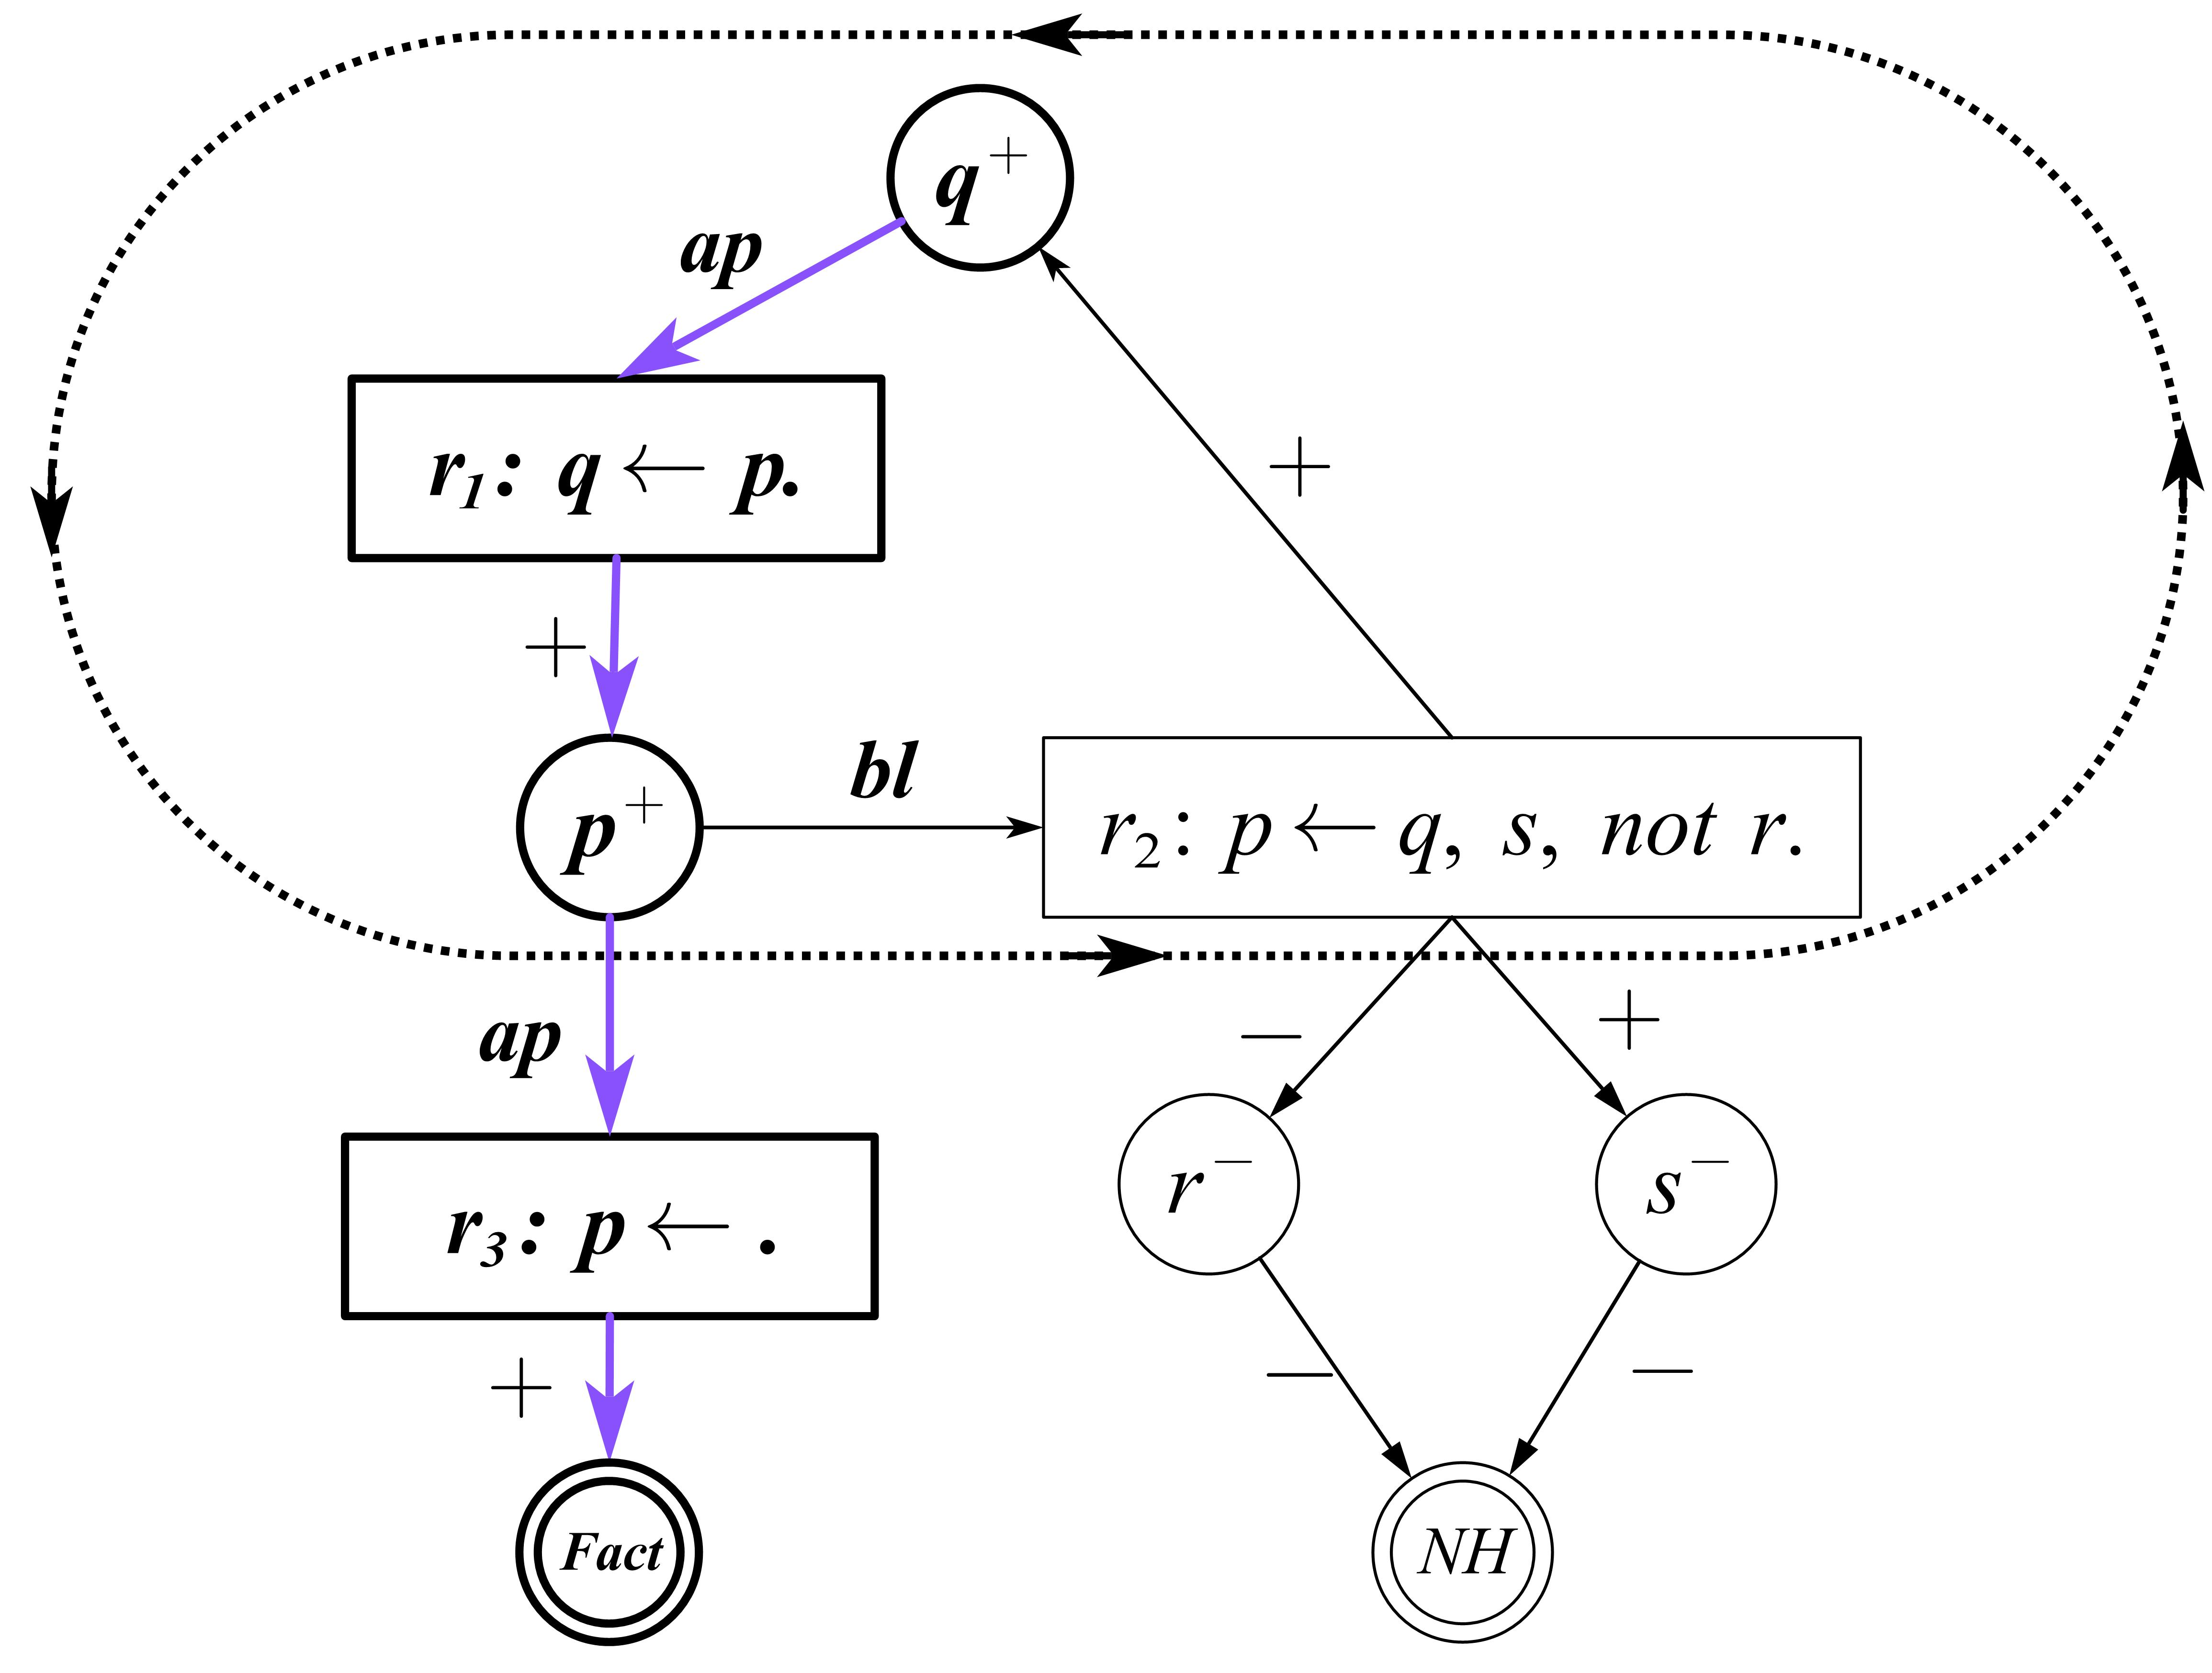
\includegraphics[height=.35\textwidth, valign=c]{figures/扩展原子规则图.jpg}} 
    \quad\quad
    \subfloat[扩展原子-规则图$ARG^{\{r\}}_{P_3}$]{\includegraphics[height=.35\textwidth, valign=c]{figures/扩展原子规则图_new.pdf}} 
    \caption{程序\hyperref[prg:p3]{$P_3$}的原子-规则图与扩展原子-规则图} 
    \label{fig:3_3} 
\end{figure}
\section{ASP扩展原子-规则图的环处理}
为了处理扩展原子-规则图中的环,首先给出扩展原子-规则图中环的形式化定义。
\begin{definition}[扩展原子-规则图中的环]
    给定一个实例化的一致性ASP程序$P$及$P$的一个回答集$M \in SM(P)$,$P$在$M$下的扩展原子图$ARG_P^M= \langle V, E \rangle$中的一条非空路径$e_1, e_2, \ldots, e_n, (e_i \in E)$对应的顶点序列为$v_1, v_2, \ldots, v_n, v_1$,其中$e_i (1 \le i \le n-1)$是从$v_i$指向$v_{i+1}$的有向边,$e_n$是从$v_n$指向$v_1$的有向边。若$\forall i \neq j \in 1 \ldots n, v_i \neq v_j$,则称该路径为$ARG_P^M$中的环,记为$cyc(P,M)$,表示为$v_1 \rightarrow v_2 \rightarrow \ldots v_{n-1} \rightarrow v_n \rightarrow v_1$。如不做特别说明,本文使用$cyc(P,M)$表示$ARG_P^M$中的一个环,必要时对一张图内不同的环使用下标加以区分。对任意的环$cyc_i(P,M)$,如果其中的所有规则依赖边均标记为“+”,称这样的环为\textbf{正环},将其记作$cyc_i^+(P,M)$,否则称为\textbf{负环},记作$cyc_i^-(P,M)$。
\end{definition}

\begin{example}[扩展原子-规则图中的环]
    如图\ref{fig:3_3}(b)所示,程序\hyperref[prg:p3]{$P_3$}关于回答集$\{r\}$的扩展原子-规则图中有两个环:负环$s^+ \rightarrow r_1 \rightarrow r^- \rightarrow r_2 \rightarrow s^+$与正环$s^+ \rightarrow r_3 \rightarrow p^+ \rightarrow r_4 \rightarrow s^+$。
\end{example}

为了避免由于环而带来的无限解释,需要为每一个环找到一个不在环中的结点相连,这样的结点称为环的\textbf{出口},其形式化定义如下:

\begin{definition}[扩展原子-规则图环出口]
    给定一个实例化一致性ASP程序$P$及$P$的一个回答集$M \in SM(P)$,$cyc(P, M)$是其扩展原子-规则图的一个环。对$v_e \in V \setminus cyc(P, M)$,若$\exists v_i \in cyc(P,M), e_i=(v_i, v_e) \in E$且$\exists v_s \in V_{sink}, v_e$可达$v_s$,则$v_e$是$cyc(P, M)$的一个出口。
\end{definition}

\begin{example}[扩展原子-规则图环出口]
    如图\ref{fig:3_3}所示,程序\hyperref[prg:p2]{$P_2$}关于回答集$\{p, q\}$的扩展原子-规则图中的正环$q^+ \rightarrow r_1 \rightarrow p^+ \rightarrow r_2 \rightarrow q^+$有一个$r_3$结点为出口,而程序\hyperref[prg:p3]{$P_3$}关于回答集$\{r\}$的负环$s^+ \rightarrow r_1 \rightarrow r^- \rightarrow r_2 \rightarrow s^+$与正环$s^+ \rightarrow r_3 \rightarrow p^+ \rightarrow r_4 \rightarrow s^+$没有出口。
\end{example}

通过对扩展原子-规则的环及环的出口的定义,可以发现没有出口的环才是导致无限解释出现的根本原因。针对这一问题,本文进一步考虑对无出口环的处理。
\subsection{无出口负环处理}
首先,考虑负环的处理。Pontelli等人在离线解释的研究中发现,对于任意一个ASP程序$P$,其回答集$M$由集合$NANT(P) \setminus (WF^+_P \cup WF^-_P)$中元素的真值唯一决定\cite{pontelli2006justifications},其中$WF^+_P$与$WF^-_P$为程序$P$的良基模型,$NANT(P)=\{b \in At \mid \exists r \in P, s.t.\ b \in body^-(r)\}$,即程序P中所有规则负体部原子构成的集合。在离线解释的研究中,Pontelli等人提出引理如下\cite{pontelli2009justifications}:
\begin{lemma}
    \label{lma:wfnonegcycle}
    给定ASP程序$P$及其一个回答集$M$,$WF_P=WF^+_P \cup WF^-_P$是其良基模型,若$a \ in WF_P$,则$a$关于$M$的离线解释(假设集合为空)中不含有负环。
\end{lemma}

基于该引理,可以得到下面的定理\ref{thm:negatomnotinwf}:%
\begin{theorem}[负环原子不在良基模型中]
    \label{thm:negatomnotinwf}
    给定ASP程序$P$及其一个回答集$M$,$WF_P=WF^+_P \cup WF^-_P$是其良基模型,对$ARG^M_P$中的任意负环$cyc^-(P, M)$,有$\forall a \in cyc^-(P, M) \cap V_{atom} \notin WF_P$。
\end{theorem}

\begin{proof}[定理\ref{thm:negatomnotinwf}的证明]
    考虑引理\ref{lma:wfnonegcycle}的逆否命题:给定ASP程序$P$及其一个回答集$M$,$WF_P=WF^+_P \cup WF^-_P$是其良基模型,若$a \in At$关于$M$的离线解释(假设集合为空)中含有负环,则$a \notin WF_P$。而$ARG^M_P$中的负环与离线解释中的负环相比,仅多出了文字结点间的显式规则结点,因此$ARG^M_P$中负环内的文字$a$一定不在良基模型中。
\end{proof}

根据定理\ref{thm:negatomnotinwf},结合负环的定义,可以将负环待处理文字的范围缩减为$NANT(P) \setminus (WF^+_P \cup WF^-_P)$中的原子。实际上,这些原子在良基语义模型构建过程中被赋值为“未定义”。当$WF^+_P \cup WF^-_P = At(P)$时,称良基模型是完全的,此时良基模型与回答集是重合的。于是考虑对程序进行修改,对不在良基模型中文字的真值作出“强制为假的假设”,使得修改后的程序具有完全的良基模型,这时程序中的各文字的解释将不会出现负环。在面向用户的解释中,为了最大程度地给用户提供交互,需要找出所有备选的假设集合,该集合满足:当通过改变程序强制使得集合中其中的文字为假时,变换后的程序具有完备的良基模型。这里提到的“强制为假”的程序变换称为负规约(negative reduct,NR),定义如下:
\begin{definition}[负规约]
    给定一个实例化的一致性一般逻辑程序$P$,$U \subseteq At$为一系列程序中原子的集合,则$P$在集合$U$下的负规约$NR(P, U)$定义为
    \begin{align}
        NR(P, U) = \{r \in P \mid head(r) \notin U\}
    \label{eq:nrpu}
    \end{align}
\end{definition}
于是程序$P$在回答集$M$下备选的假设集的集合$ASM(P,M)$定义为:
\begin{align}
    ASM(P, M) = \{U \subseteq NANT(P) \mid (U \cap M = \emptyset) \land (U \notin WF^+_P \cup WF^-_P) \land WF^+_{NR(P,U)}=M\}
\label{eq:asm}
\end{align}

式\eqref{eq:nrpu}对程序进行的负规约实际上是通过去掉程序$P$中头部在$U$中的所有规则,以使得剩余程序$NR(P, U)$无法推出$U$中文字。而式\eqref{eq:asm}试图找到同时满足如下几个条件的假设集:
\begin{itemize}[topsep=0pt]
    \setlength\itemsep{-0.3em}
    \item 集合中的所有原子来源于程序中的负体部
    \item 集合中的所有原子不在回答集中
    \item 集合中的所有原子不在良基模型中
    \item 在该集合下对程序进行负规约后,程序的良基模型与回答集重合
\end{itemize}
在这种情况下,将$ASM(P,M)$中任意一个集合中原子的不正确解释为“假定”,一方面能够打破原有解释中的负环,另一方面也还原了回答集构建过程中固有的猜测过程。下面通过程序\hyperref[prg:p_4]{$P_4$}对上述负环的处理进行说明。
\begin{example}[程序\texorpdfstring{\hyperref[prg:p_4]{$P_4$}})]
    考虑程序$P_4$:
    \begin{center}
        \begin{tabular*}{\linewidth}{rl@{\extracolsep{\fill}}ll}
        \label{prg:p_4}
          &$r_1: a \leftarrow.$ &$r_2: c \leftarrow a, not\ b.$ & $r_3: b \leftarrow not\ c.$\\ 
          &$r_4: e \leftarrow not\ d.$ &$r_5: f \leftarrow e.$ &$r_6: f \leftarrow not\ a.$
        \end{tabular*}
    \end{center}
    程序\hyperref[prg:p_4]{$P_4$}的良基模型的构建示意如图\ref{fig:3_4}所示。其良基模型最终计算为$\langle \{a,e,f\}, \{d\} \rangle$,$\{b, c\}$为“undefined”,其稳定语义模型有两个,分别为$M_1=\{a,e,f,b\}$与$M_2=\{a,e,f,c\}$。
    \begin{figure}[htbp]
        \centering 
        \includegraphics[height=.63\textwidth, valign=c]{figures/wfm计算.pdf}
        \caption{程序\hyperref[prg:p_4]{$P_4$}的良基模型计算过程示意}
        \label{fig:3_4}
    \end{figure}
    
    下面考虑该程序在两个回答集下扩展的原子-规则图$ARG^{M_1}_{P_4}$与$ARG^{M_2}_{P_4}$,如图\ref{fig:3_5}(a)与图\ref{fig:3_5}(b)所示。可以看到,在良基模型之外的$b$与$c$在稳定语义模型下通过多个回答集进行了不同的赋值,紫色路径形成的负环中包含了$b$与$c$两个原子,当$b$或$c$中任意一个原子的真值确定后,回答集也唯一确定。
    \begin{figure}[htbp]
        \centering 
        \subfloat[扩展原子-规则图$ARG_{P_4}^{\{a,e,f,c\}}$]{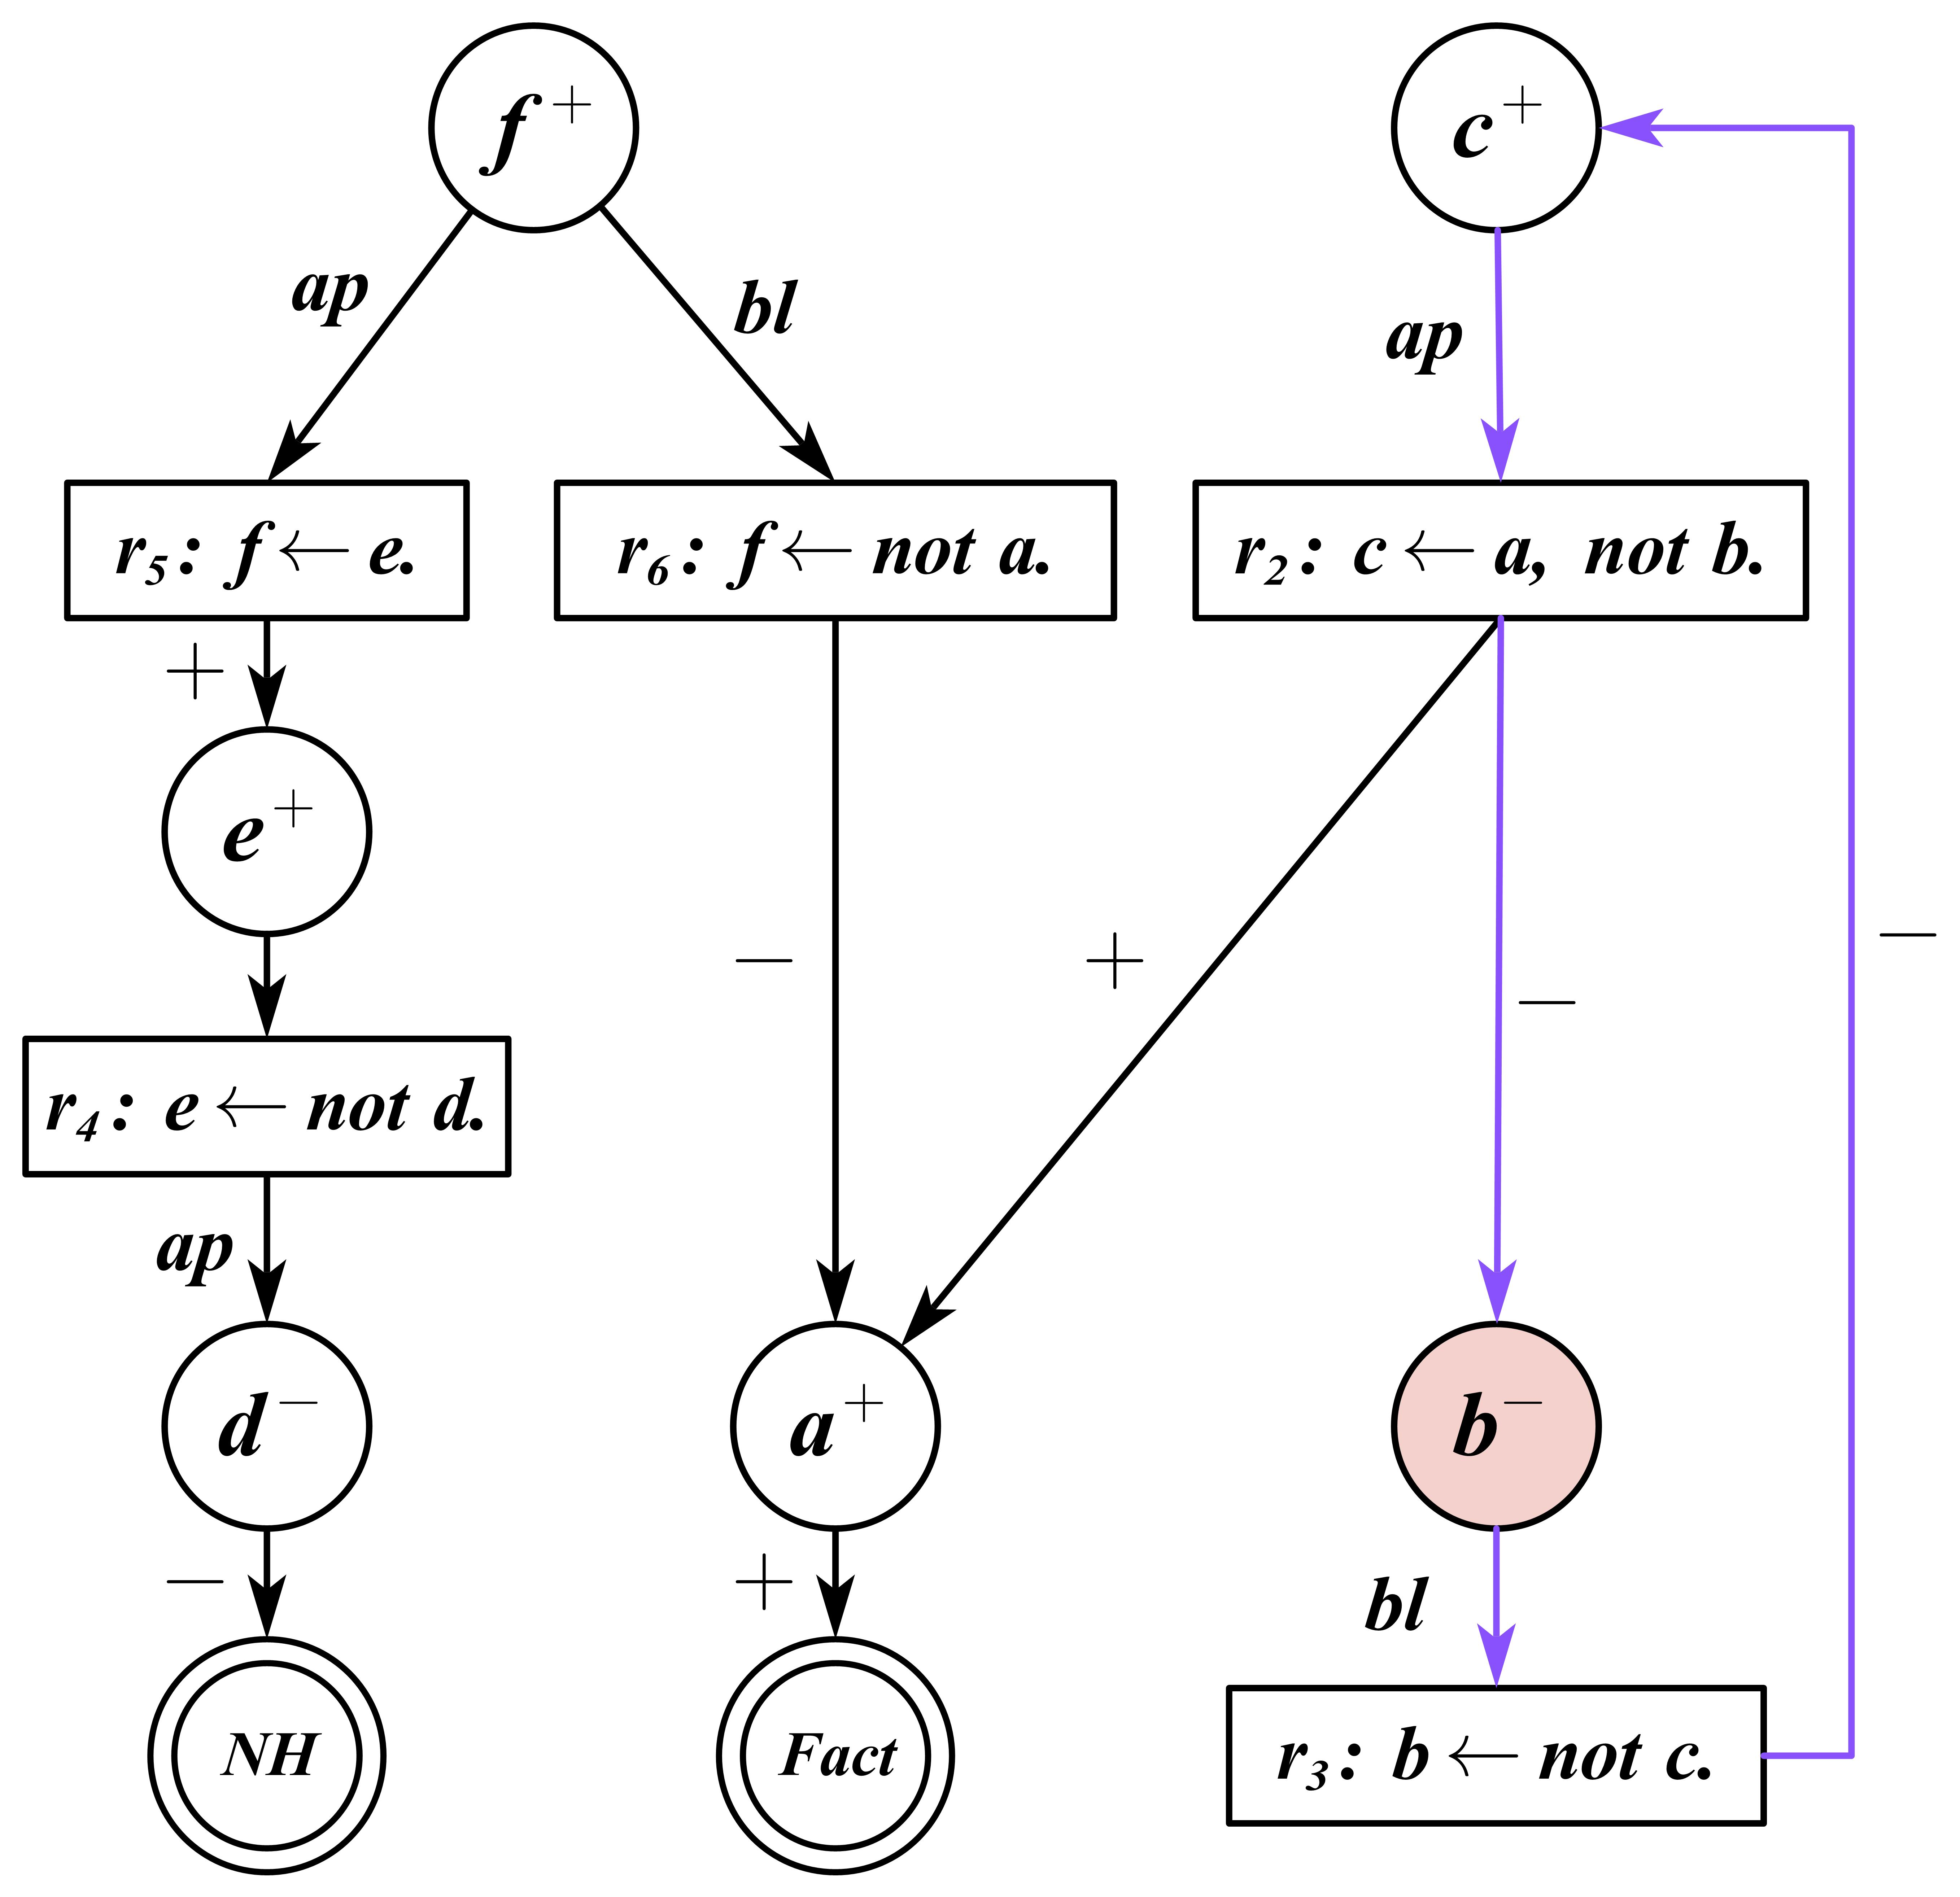
\includegraphics[height=.4\textwidth, valign=c]{figures/p4arg_m1.jpg}} 
        \quad\quad
        \subfloat[扩展原子-规则图$ARG_{P_4}^{\{a,e,f,b\}}$]{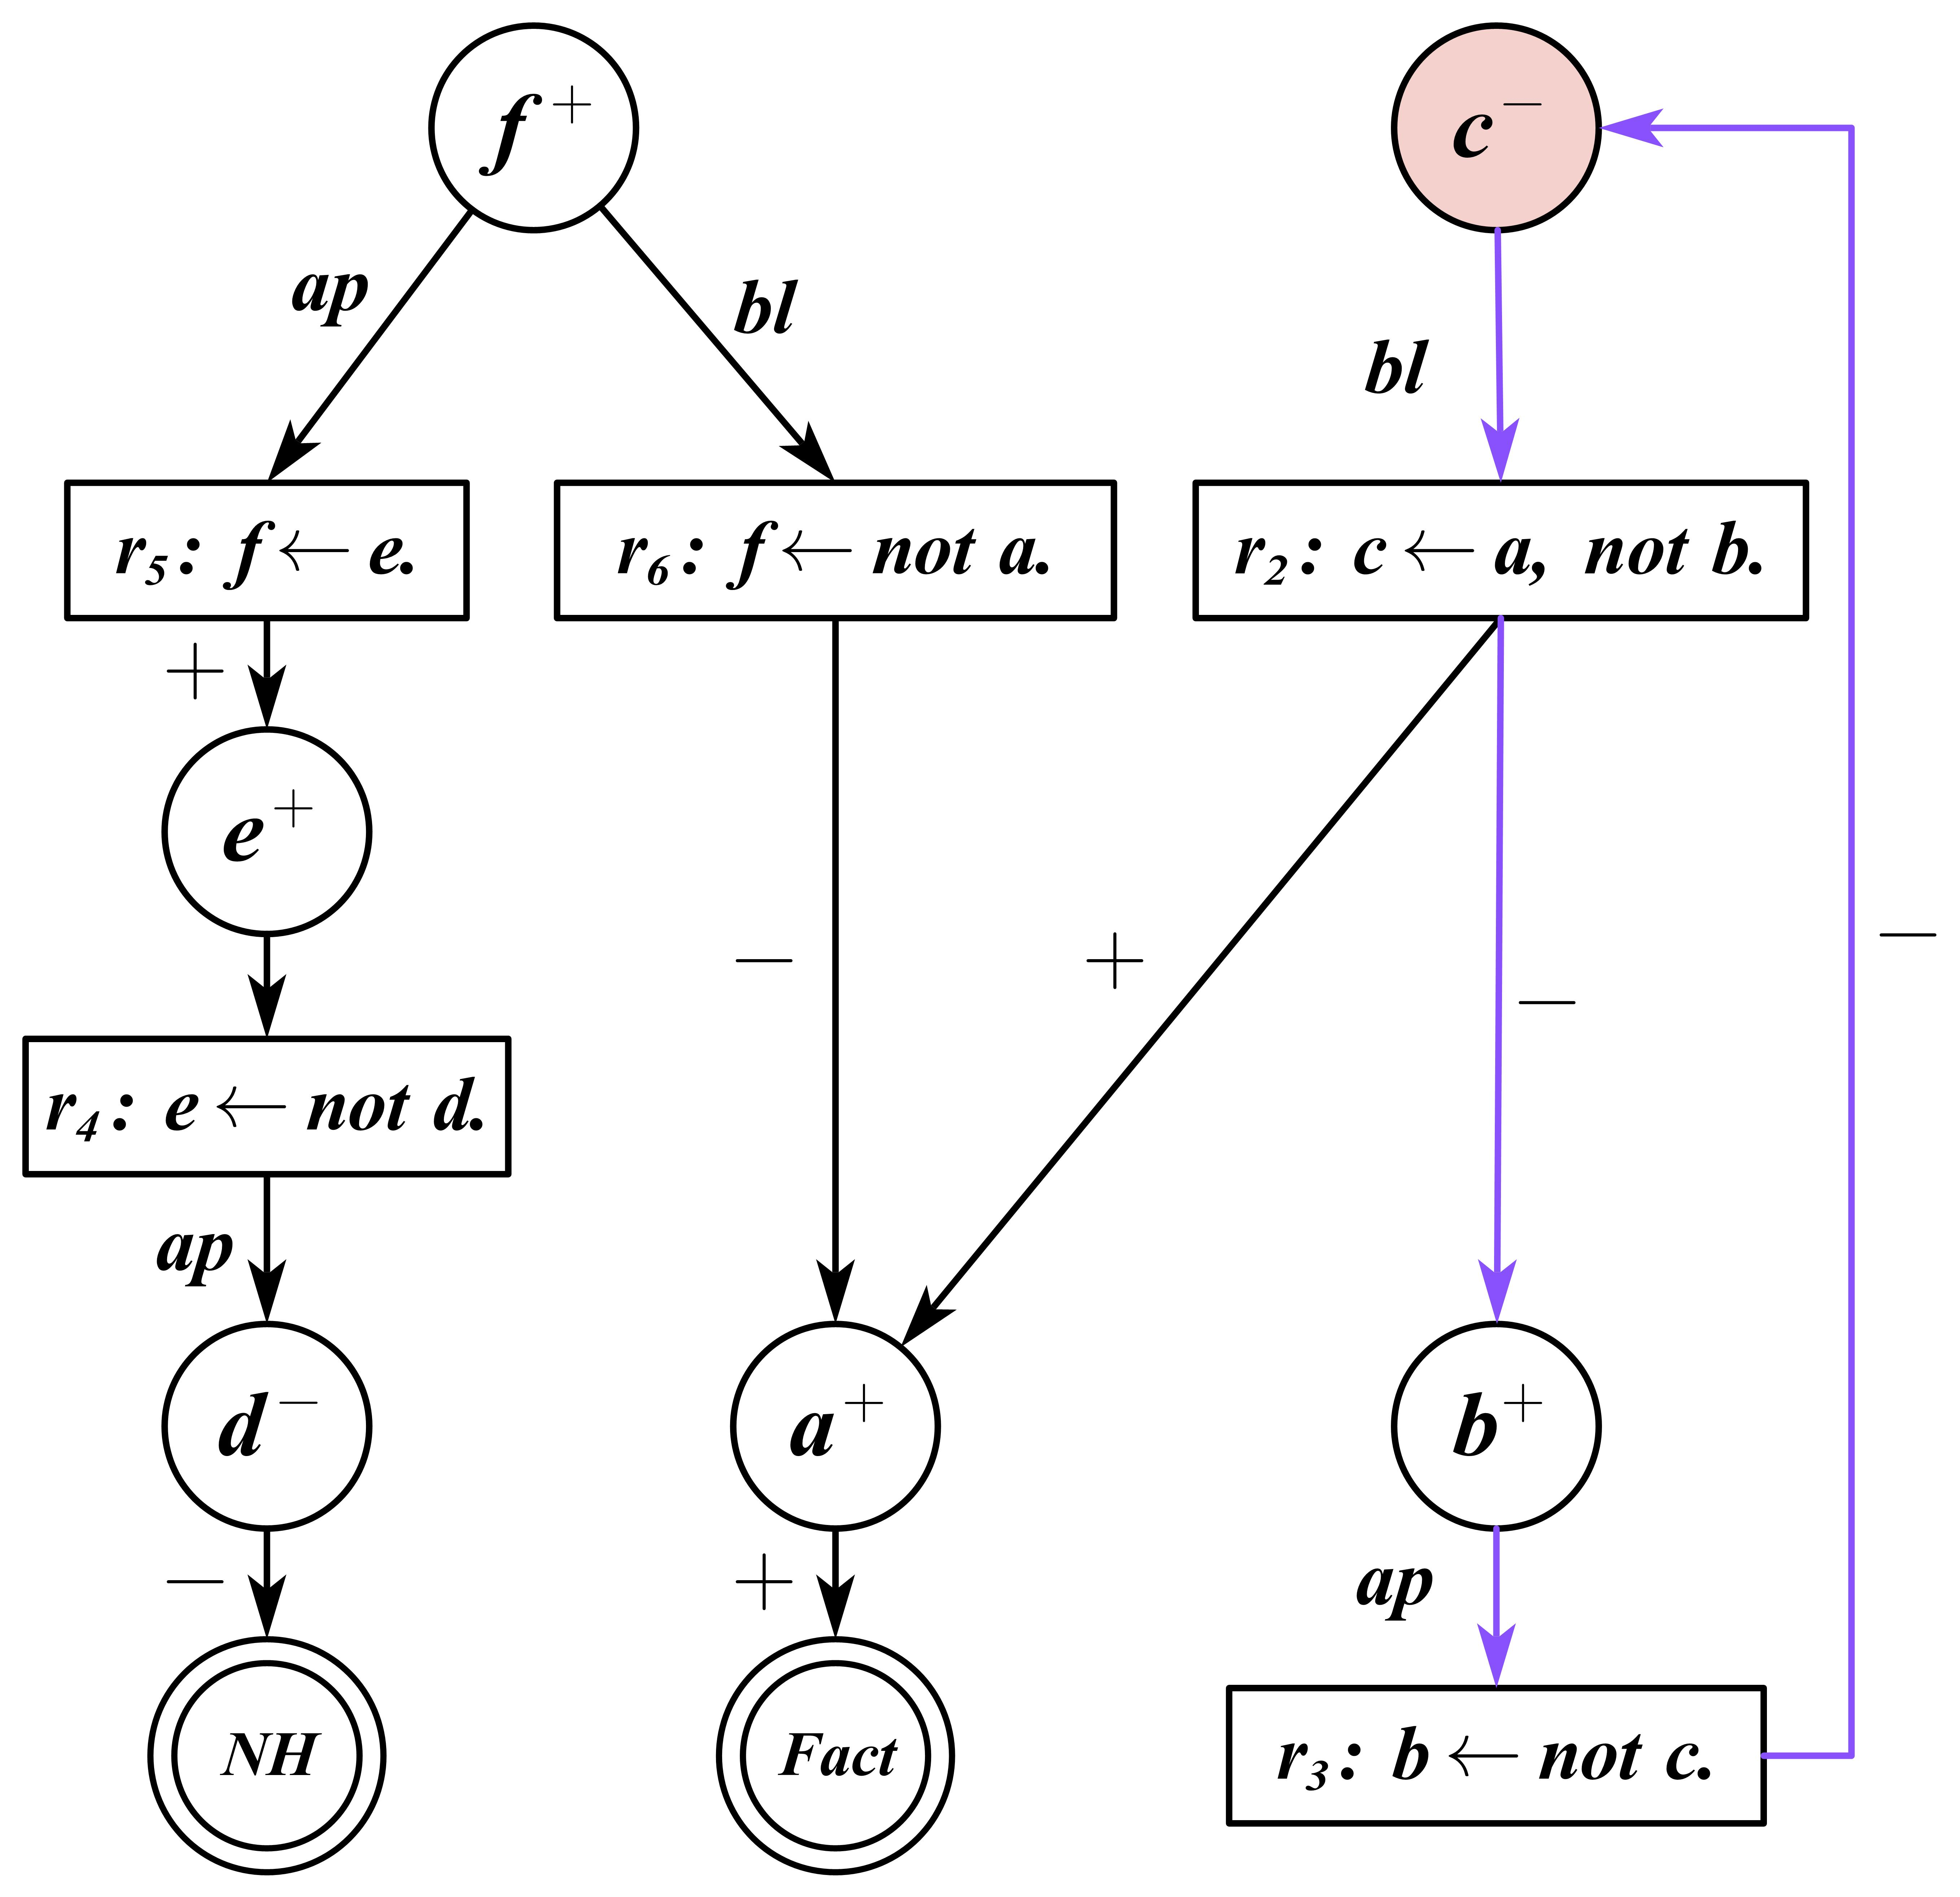
\includegraphics[height=.4\textwidth, valign=c]{figures/p4arg_m2.jpg}} 
        \caption{程序\hyperref[prg:p3]{$P_3$}的原子-规则图与扩展原子-规则图} 
        \label{fig:3_5}
    \end{figure}
    
    进一步,通过式\eqref{eq:nrpu}与\eqref{eq:asm}可以计算出备选的假设集合,其中$ASM(P_4, M_1)=\{\{b\}\}$,$ASM(P_4, M_2)=\{\{c\}\}$。
\end{example}
    需要说明的是,$ASM$集合中的元素并不一定唯一,例如程序$P_5$。
    \vspace{1ex}
    \begin{example}[程序\texorpdfstring{\hyperref[prg:p_5]{$P_5$}})]
        考虑程序$P_5$:
        \begin{center}
            \begin{tabular*}{\linewidth}{rl@{\extracolsep{\fill}}ll}
            \label{prg:p_5}
              &$r_1: p \leftarrow not\ q.$ &$r_2: q \leftarrow not\ p.$\\ 
              &$r_3: r \leftarrow not\ p.$ &$r_4: s \leftarrow not\ r.$
            \end{tabular*}
        \end{center}
        程序\hyperref[prg:p_5]{$P_5$}的良基模型计算为$\langle \emptyset, \emptyset \rangle$,所有文字均为“undefined”,其稳定语义模型有两个,分别为$M_1=\{p,s\}$与$M_2=\{q,r\}$。通过计算可以得到$ASM(P_5, M_1)=\{\{q\}, \{q, r\}\}\}$。图\ref{fig:3_6}给出了$ARG^{M_1}_{P_5}$及其环示意。此时,将$\{q\}$或$\{q,r\}$不在回答集中解释为假设为假,均能够避免在解释中出现环。
        \begin{figure}[!h]
            \centering 
            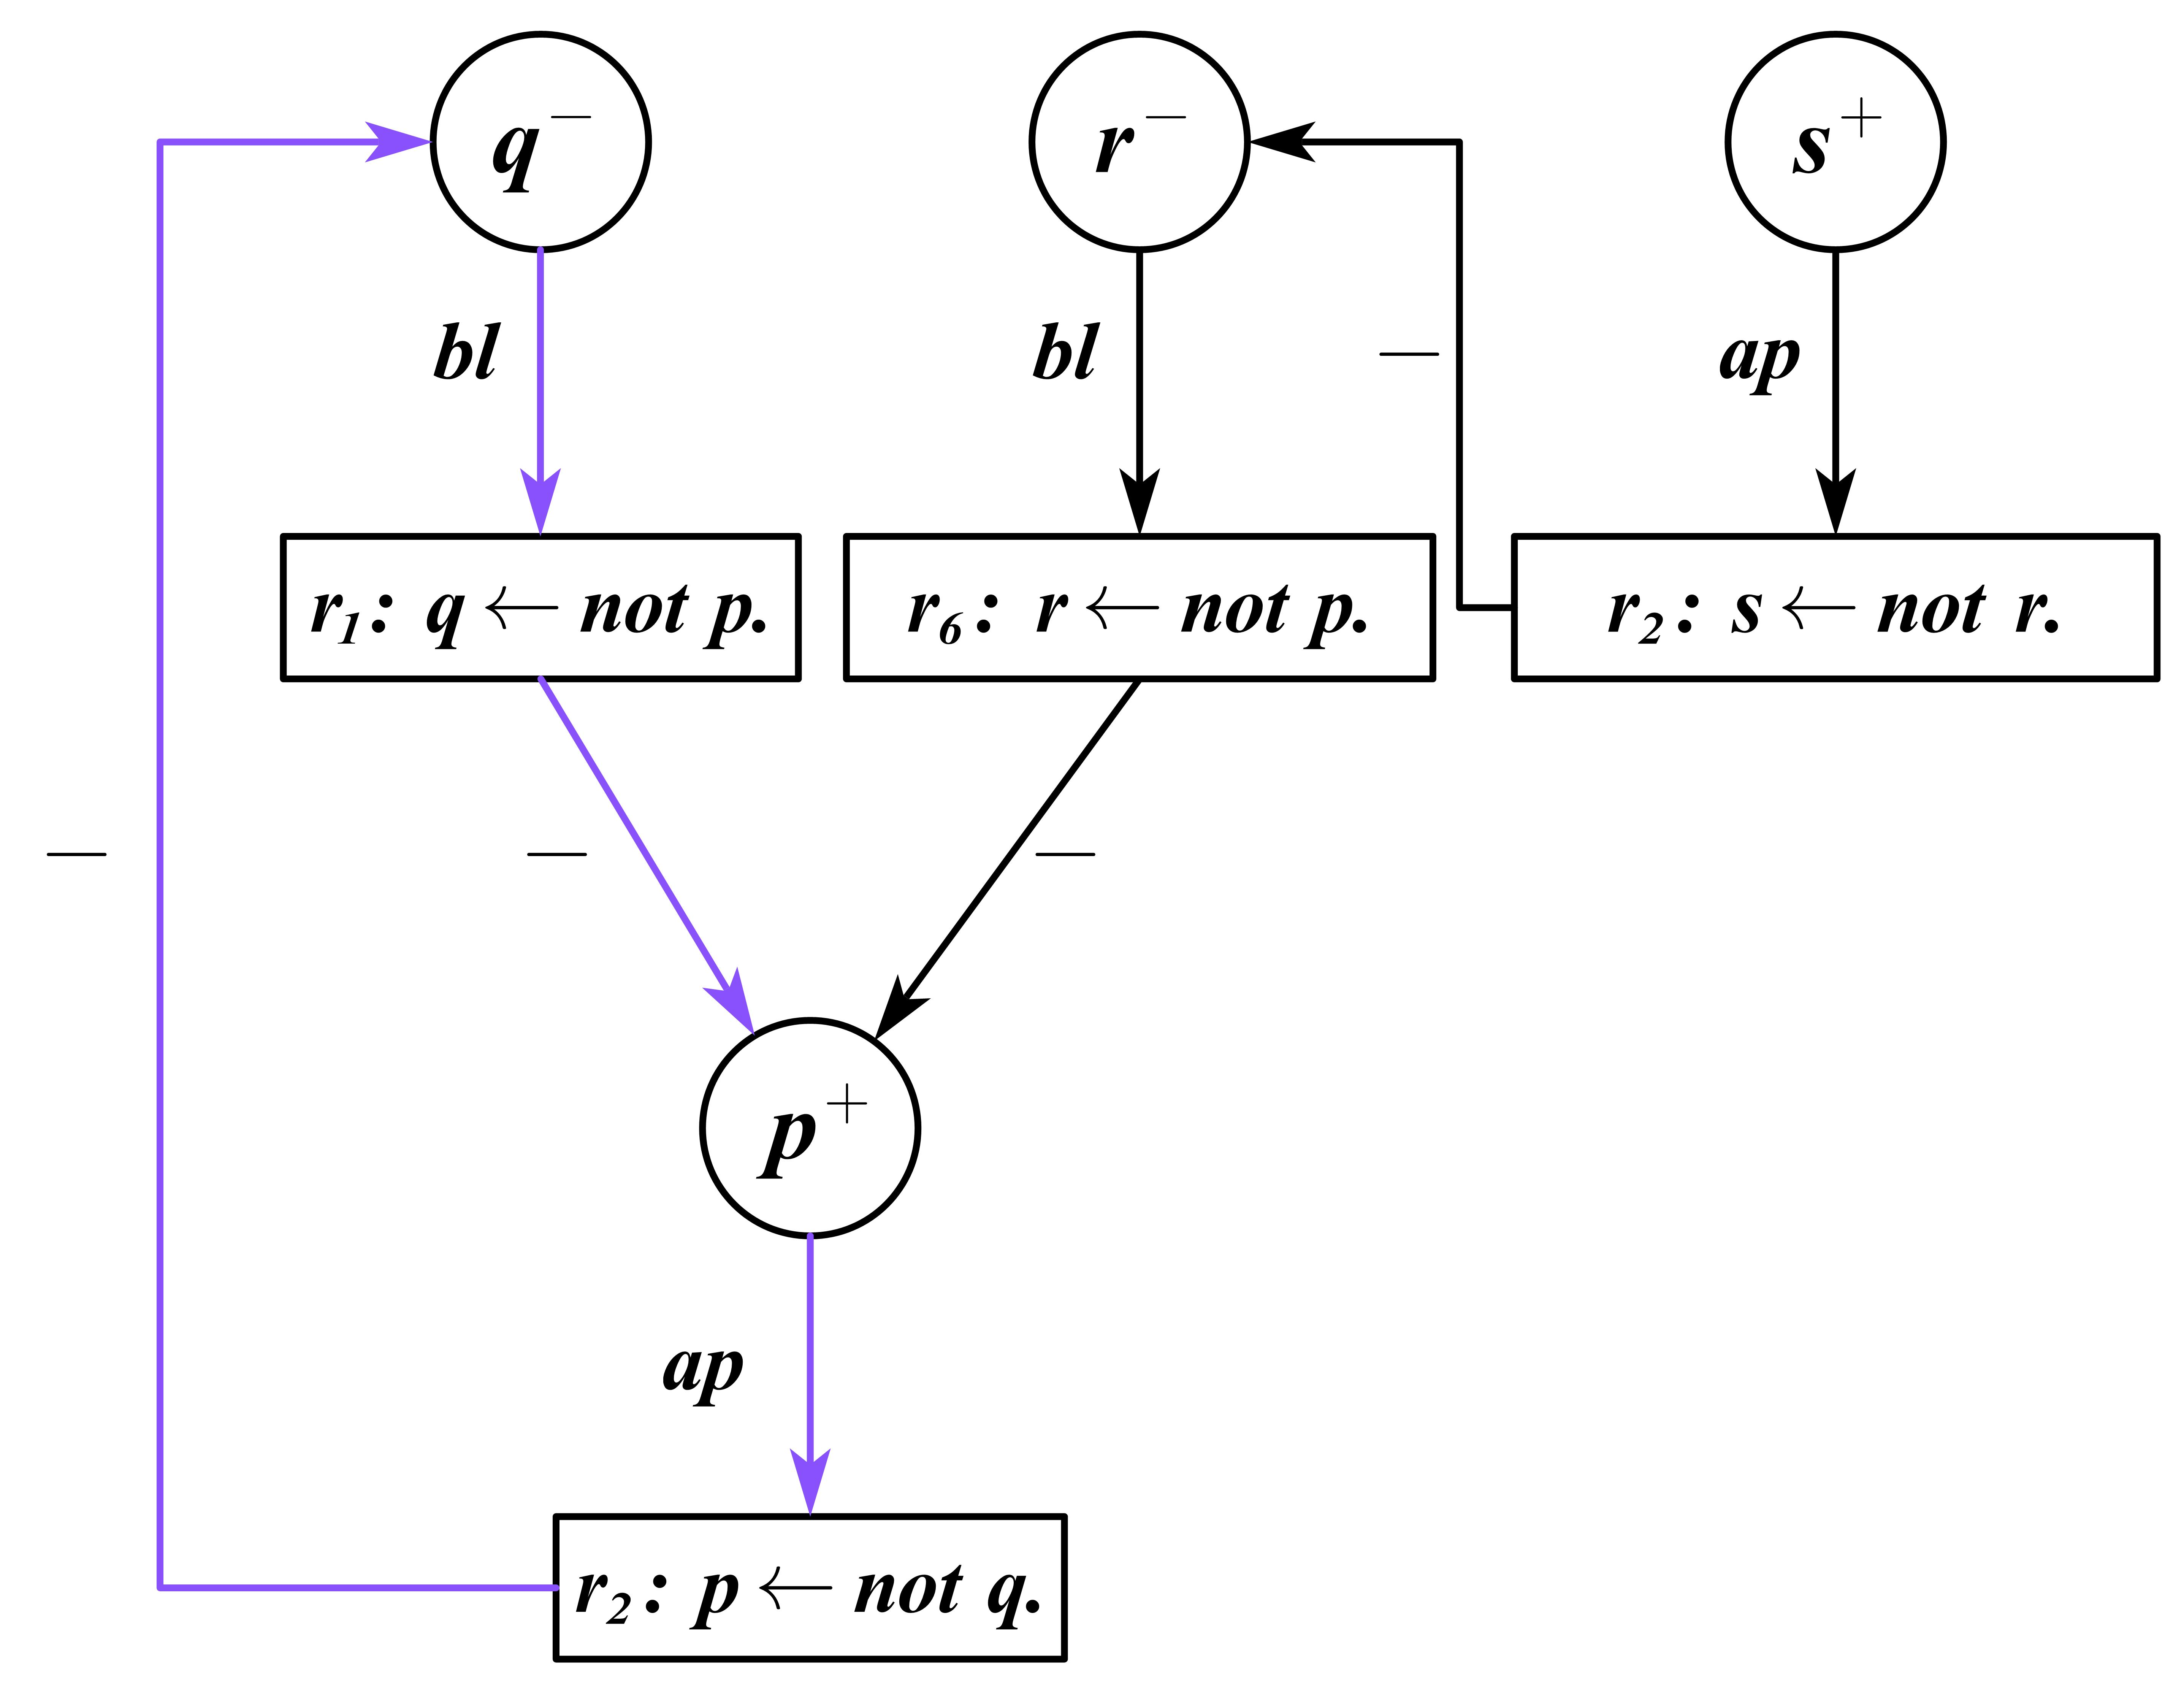
\includegraphics[height=.4\textwidth, valign=c]{figures/argp5m1.jpg}
            \caption{程序\hyperref[prg:p_5]{$P_5$}的扩展原子-规则图$ARG^{M_1}_{P_5}$}
            \label{fig:3_6}
        \end{figure}
    \end{example}
    事实上,上述研究展现了程序中负环的出现,是由于某些原子真值的不确定性。在二值逻辑下的稳定语义模型中,每个原子的真值或为真或为假,因此得到回答集的过程是一种固有的“猜测-验证”(Guess and Check)的过程\cite{eiterASP2009}。而通过上述$ASM$集合的定义,为找到这些原子提供了一种形式化的计算方法,同时也能够将集合中的原子为假归因于这一假设,从而不再由于负环中原子间的相互依赖而产生循环解释。
\subsection{无出口正环处理}
    解决了负环处理的问题后,本文接着对扩展原子-规则图中的正环特性进行研究。对无出口正环的分析基于Lin与Zhao等人提出的逻辑程序环公式\cite{lin2004assat},将其定义推广到扩展原子-规则图下。

\begin{definition}[正环的外部支持]
    给定一个实例化一致性ASP程序$P$及$P$的一个回答集$M \in SM(P)$,对$ARG^M_P$中任意的正环$cyc^+(P, M)$,记$ES_P(cyc^+(P, M))$为$cyc^+(P, M)$在程序$P$与回答集$M$下的外部支持,$EB_P(cyc^+(P, M))$为$cyc^+(P, M)$在程序$P$与回答集$M$下的外部体部集,定义如下:
    \begin{align}
        &\mathit{ES_P(cyc^+(P, M)) = \{ r \in P \mid head(r) \in cyc^+(P, M), body^+(r) \cap cyc^+(P, M) = \emptyset\}}\\
        &\mathit{EB_P(cyc^+(P, M)) = \{body(r) \mid r \in ES_P(cyc^+(P, M)) \}}
      \end{align}
\end{definition}
\begin{example}
    程序\hyperref[prg:p3]{$P_3$}在回答集$\{s, p\}$下的正环$cyc^+(P_3, \{r\})=s^+ \rightarrow r_3 \rightarrow p^+ \rightarrow r_4 \rightarrow s^+$的外部支持$ES_P(cyc^+(P_3, \{r\}))=\{r_1\}$,外部体部集为$EB_P(cyc^+(P_3, \{r\}))=\{not\ r\}$,由于$\{not\ r\}$成立,该环得到了外部支持,环内个文字均成立;而其在另一个回答集$\{r\}$下的正环$cyc+(P_3, \{r\})=s^- \rightarrow r_1 \rightarrow p^- \rightarrow r_4 \rightarrow s^-$的外部支持与$cyc^+(P_3, \{r\})$相同,但由于在该回答集下,$\{not\ r\}$不成立,该环没有得到外部支持,因此$s$与$r$在该回答集下均不成立。
\end{example}

显然,当正环的至少一条外部支持规则适用时,规则头部成立,正环内的文字得到支持;如果所有的外部支持规则都不适用,则正环内的文字无法得到支持,环内所有文字均不成立。这一结论被形式化地定义为环公式:

\begin{definition}[正环的环公式]
    给定一个ASP程序$P$及$P$的一个回答集$M \in SM(P)$,$r\in P$是其中的一条规则,定义$BF(body(r))$为规则$r$正体部与负体部文字的合取,即
    \begin{align}
        BF(body(r))=\bigwedge_{l \in body^+(r)} l \land \bigwedge_{l \in body^-(r)} \lnot l
      \end{align}
    正环$cyc^+(P, M)$的环公式定义为:
    \begin{align}
        \begin{split}
            \mathit{LF_P(cyc^+(P, M))} &\mathit{= \left( \bigvee_{l \in cyc^+(P, M)} l \right)  \rightarrow \left(\bigvee_{body(r)\in EB_P(cyc^+(P, M))}BF(body(r))\right)}\\ 
        &\mathit{\equiv  \left(\bigwedge_{body(r) \in EB_P(cyc^+(P, M))} \lnot BF(body(r)) \right) \rightarrow  \left( \bigwedge_{l \in cyc^+(P, M)} \lnot l \right)} \label{eq:loopformula}
        \end{split}
        \end{align}
\end{definition}

式\eqref{eq:loopformula}中可以看到,对于任意一个正环而言,如果环外的规则都不能被适用,那么环内所有文字均不正确。Pontelli等人在离线解释研究中的发现,离线解释图中的环(负环已通过$ASM$集合假设进行处理),只可能是结点各文字均为假且相互依赖的环\cite{pontelli2009justifications},这一结论与本文的发现相一致,这里从环公式的视角再次印证了这一结论。因此,本文将这一性质作为正环内文字均为假的原因并在解释中呈现。

\section{ASP程序解释空间及其构建算法设计}
\subsection{ASP程序解释空间定义}
在处理完程序中的没有出口的正环与负环后,本文对扩展原子-规则图$ARG$进一步改进,提出ASP程序的解释空间(Explanation Universe,EU),具体定义如下:
\begin{definition}[ASP程序解释空间]
    给定一个一致的ASP程序$P$及其一个回答集$M \in SM(P)$,程序$P$在$M$下的解释空间基于$ARG^P_M$定义,在其基础上作出如下修改:
    \begin{itemize}[topsep=0pt]
        \setlength\itemsep{-0.3em}
        \item $V_{sink} = V_{sink} \cup \{ASM\} \cup \{UE\}$,即扩充定义两个新类型的汇结点,其中$ASM$表示“假设为假”,$UE$表示未得到外部支持;
        \item $E_{end} = E_{end} \cup E_{ue} \cup E_{asm}$,即在终结边的基础上增加两种新的边:
        \begin{itemize}[topsep=0pt,label=$\circ$]
            \setlength\itemsep{-0.3em}
            \item $E_{ue} = \{(v, -, UE) \mid v \in cyc^+(P, M), cyc^+(P, M)\text{ 未受到外部支持}\}$
            \item $E_{end} = \{(v, -, ASM) \mid v \in cyc^-(P, M), \exists U \in ASM(P, M), v \in U\}$
        \end{itemize}
    \end{itemize}
\end{definition}

\begin{example}[程序\texorpdfstring{\hyperref[prg:p_4]{$P_4$}})]
    程序$P_4$的两个回答集分别是$M_1=\{p,s\}$与$M_2=\{r\}$。在$\{p,s\}$下计算得到的备选假设集为$\{\{r\}\}$,而在$\{r\}$下计算得到的备选假设集为$\{\{s\}, \{p,s\}\}$。图\ref{fig:3_7}(a)中,橘黄色路径构成一个未被外部支持的正环,因此$s^-$与$p^-$均与$UE$结点相连,同时该解释空间对$\{s\}$为假作出基于假设的解释,因此$s^-$与$ASM$结点相连;图\ref{fig:3_7}(b)中,橘黄色路径构成的正环得到了外部规则$r_1$的支持,因此$s^-$与$p^-$均与$UE$结点相连,同时该解释空间对$\{r\}$为假作出基于假设的解释,因此$r^-$与$ASM$结点相连。
    \begin{figure}[htbp]
        \centering 
        \subfloat[程序$P_4$的解释空间$EU^{P_4}_{\{r\}, \{s\}}$]{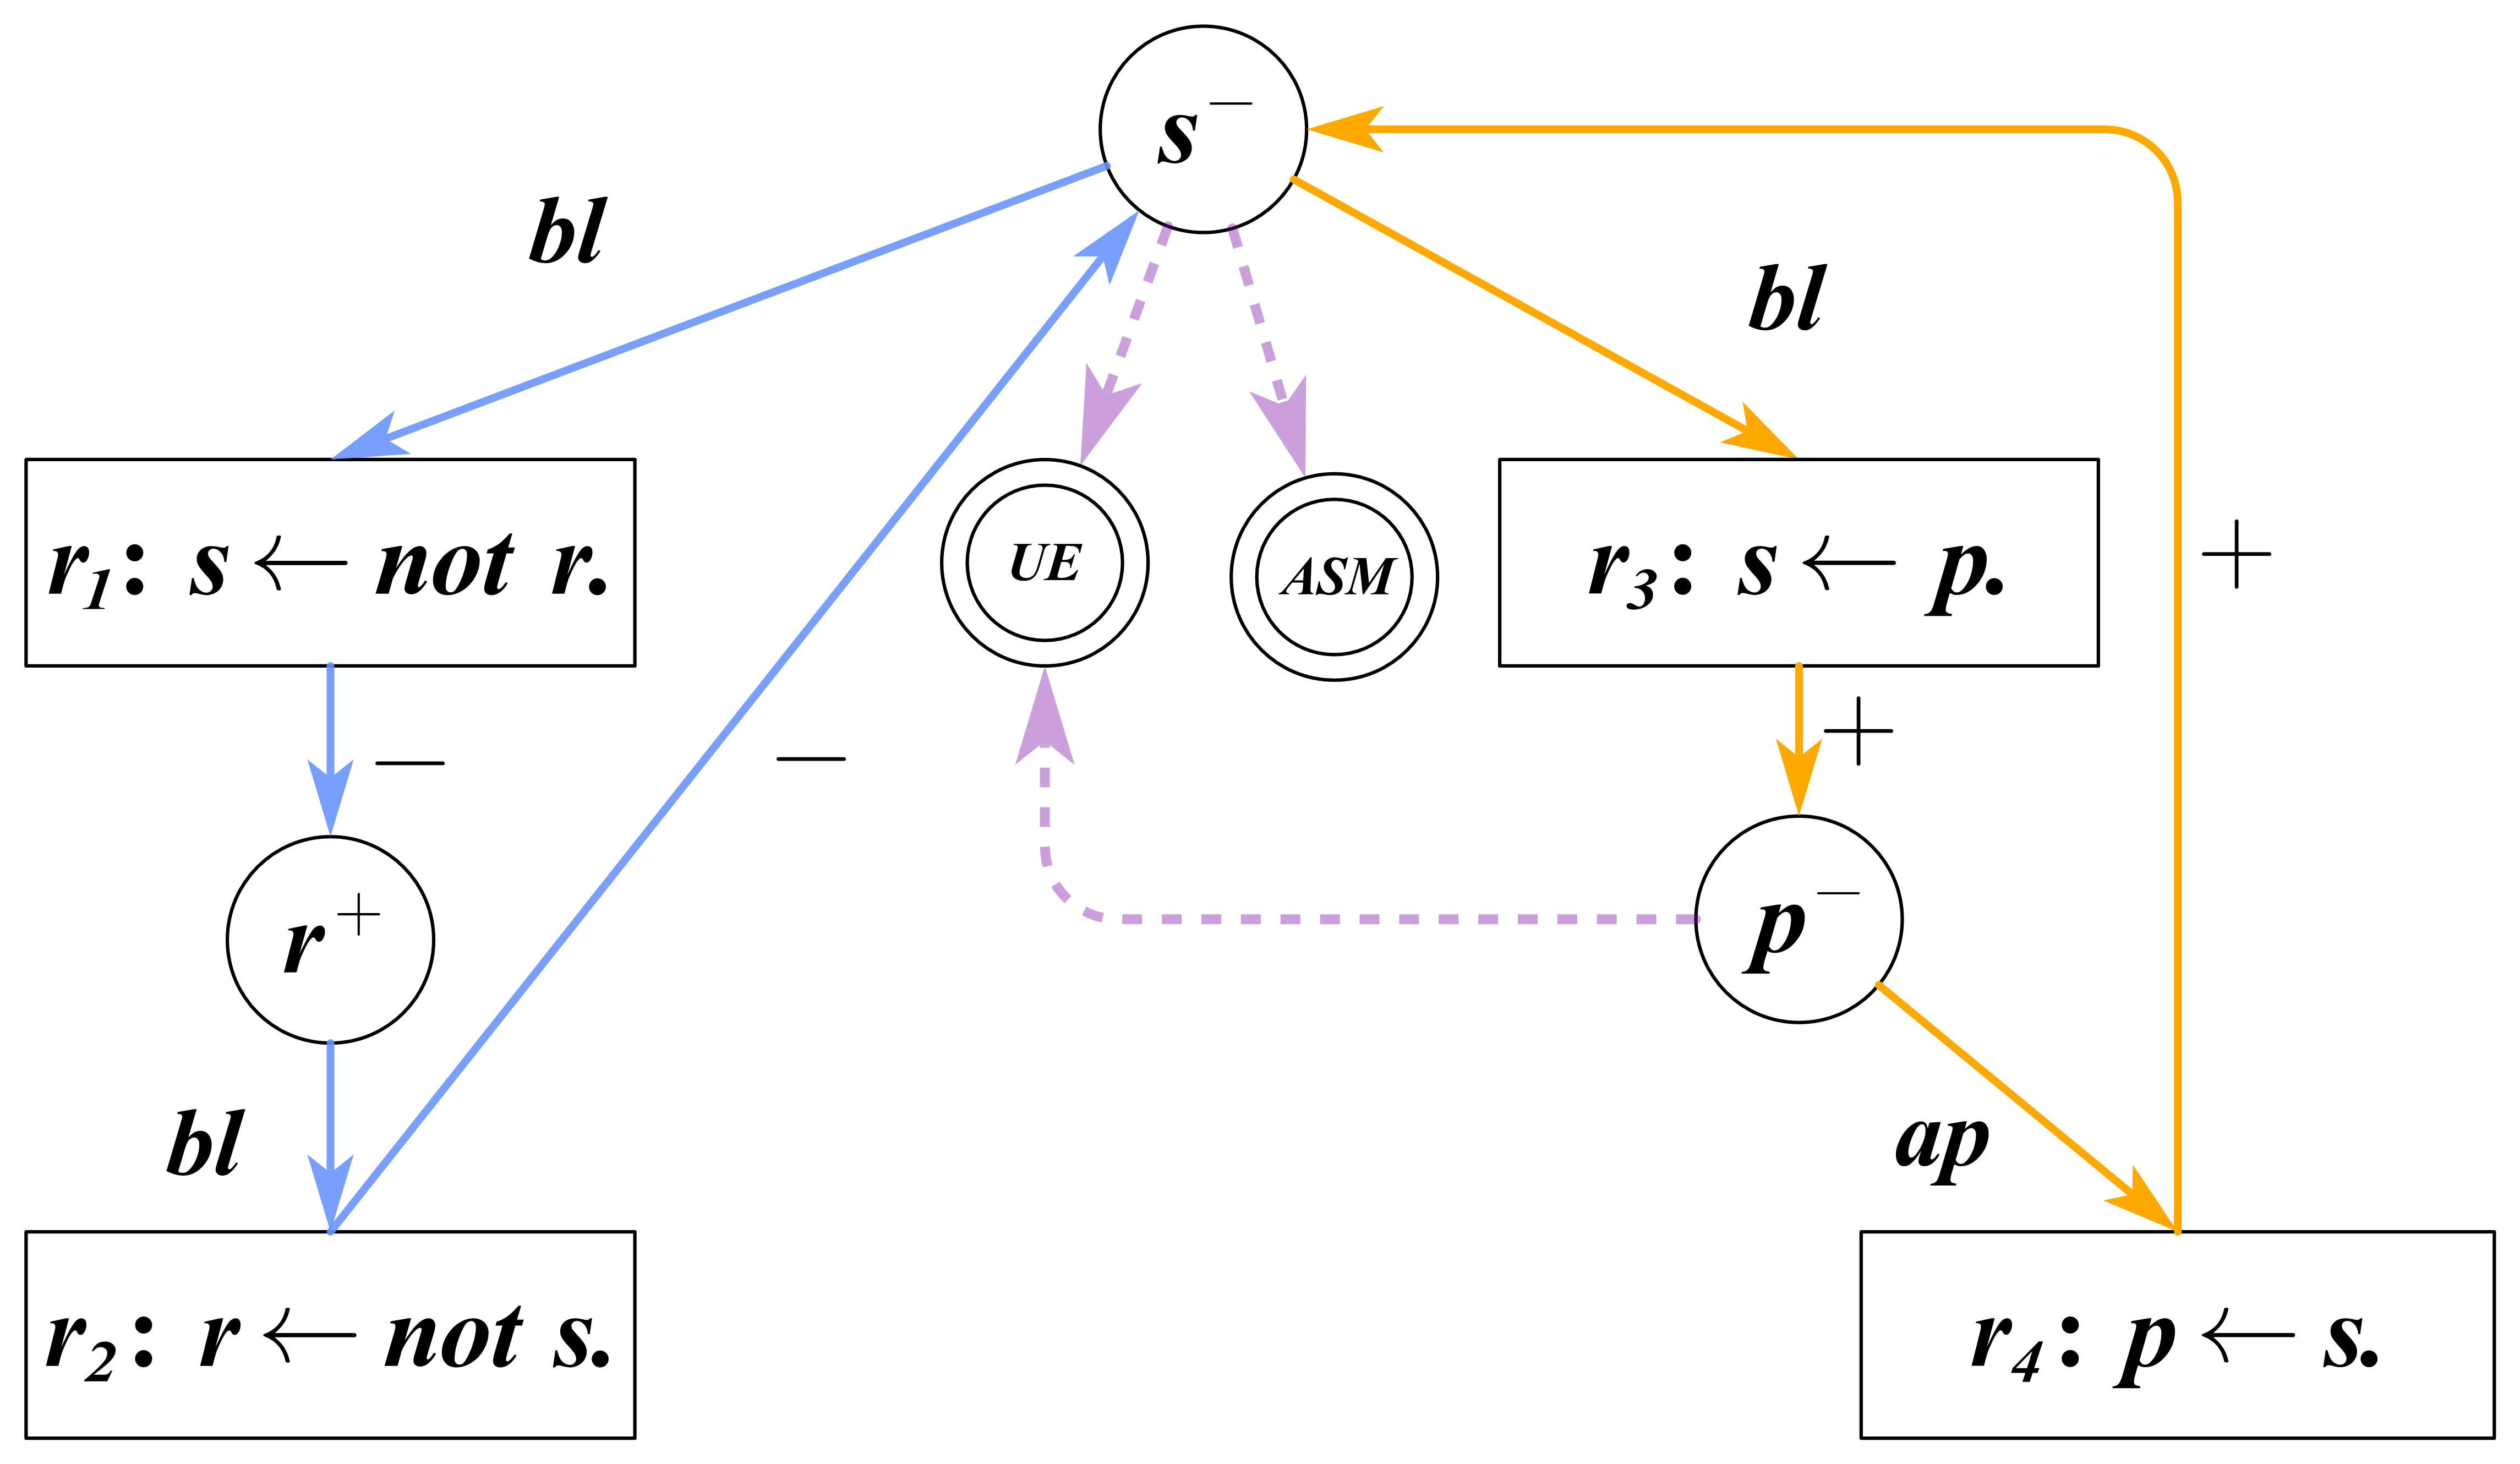
\includegraphics[height=.25\textwidth, valign=c]{figures/解释空间_1.jpg}} 
        \quad\quad
        \subfloat[程序$P_4$的解释空间$EU^{P_4}_{\{p, s\}, \{r\}}$]{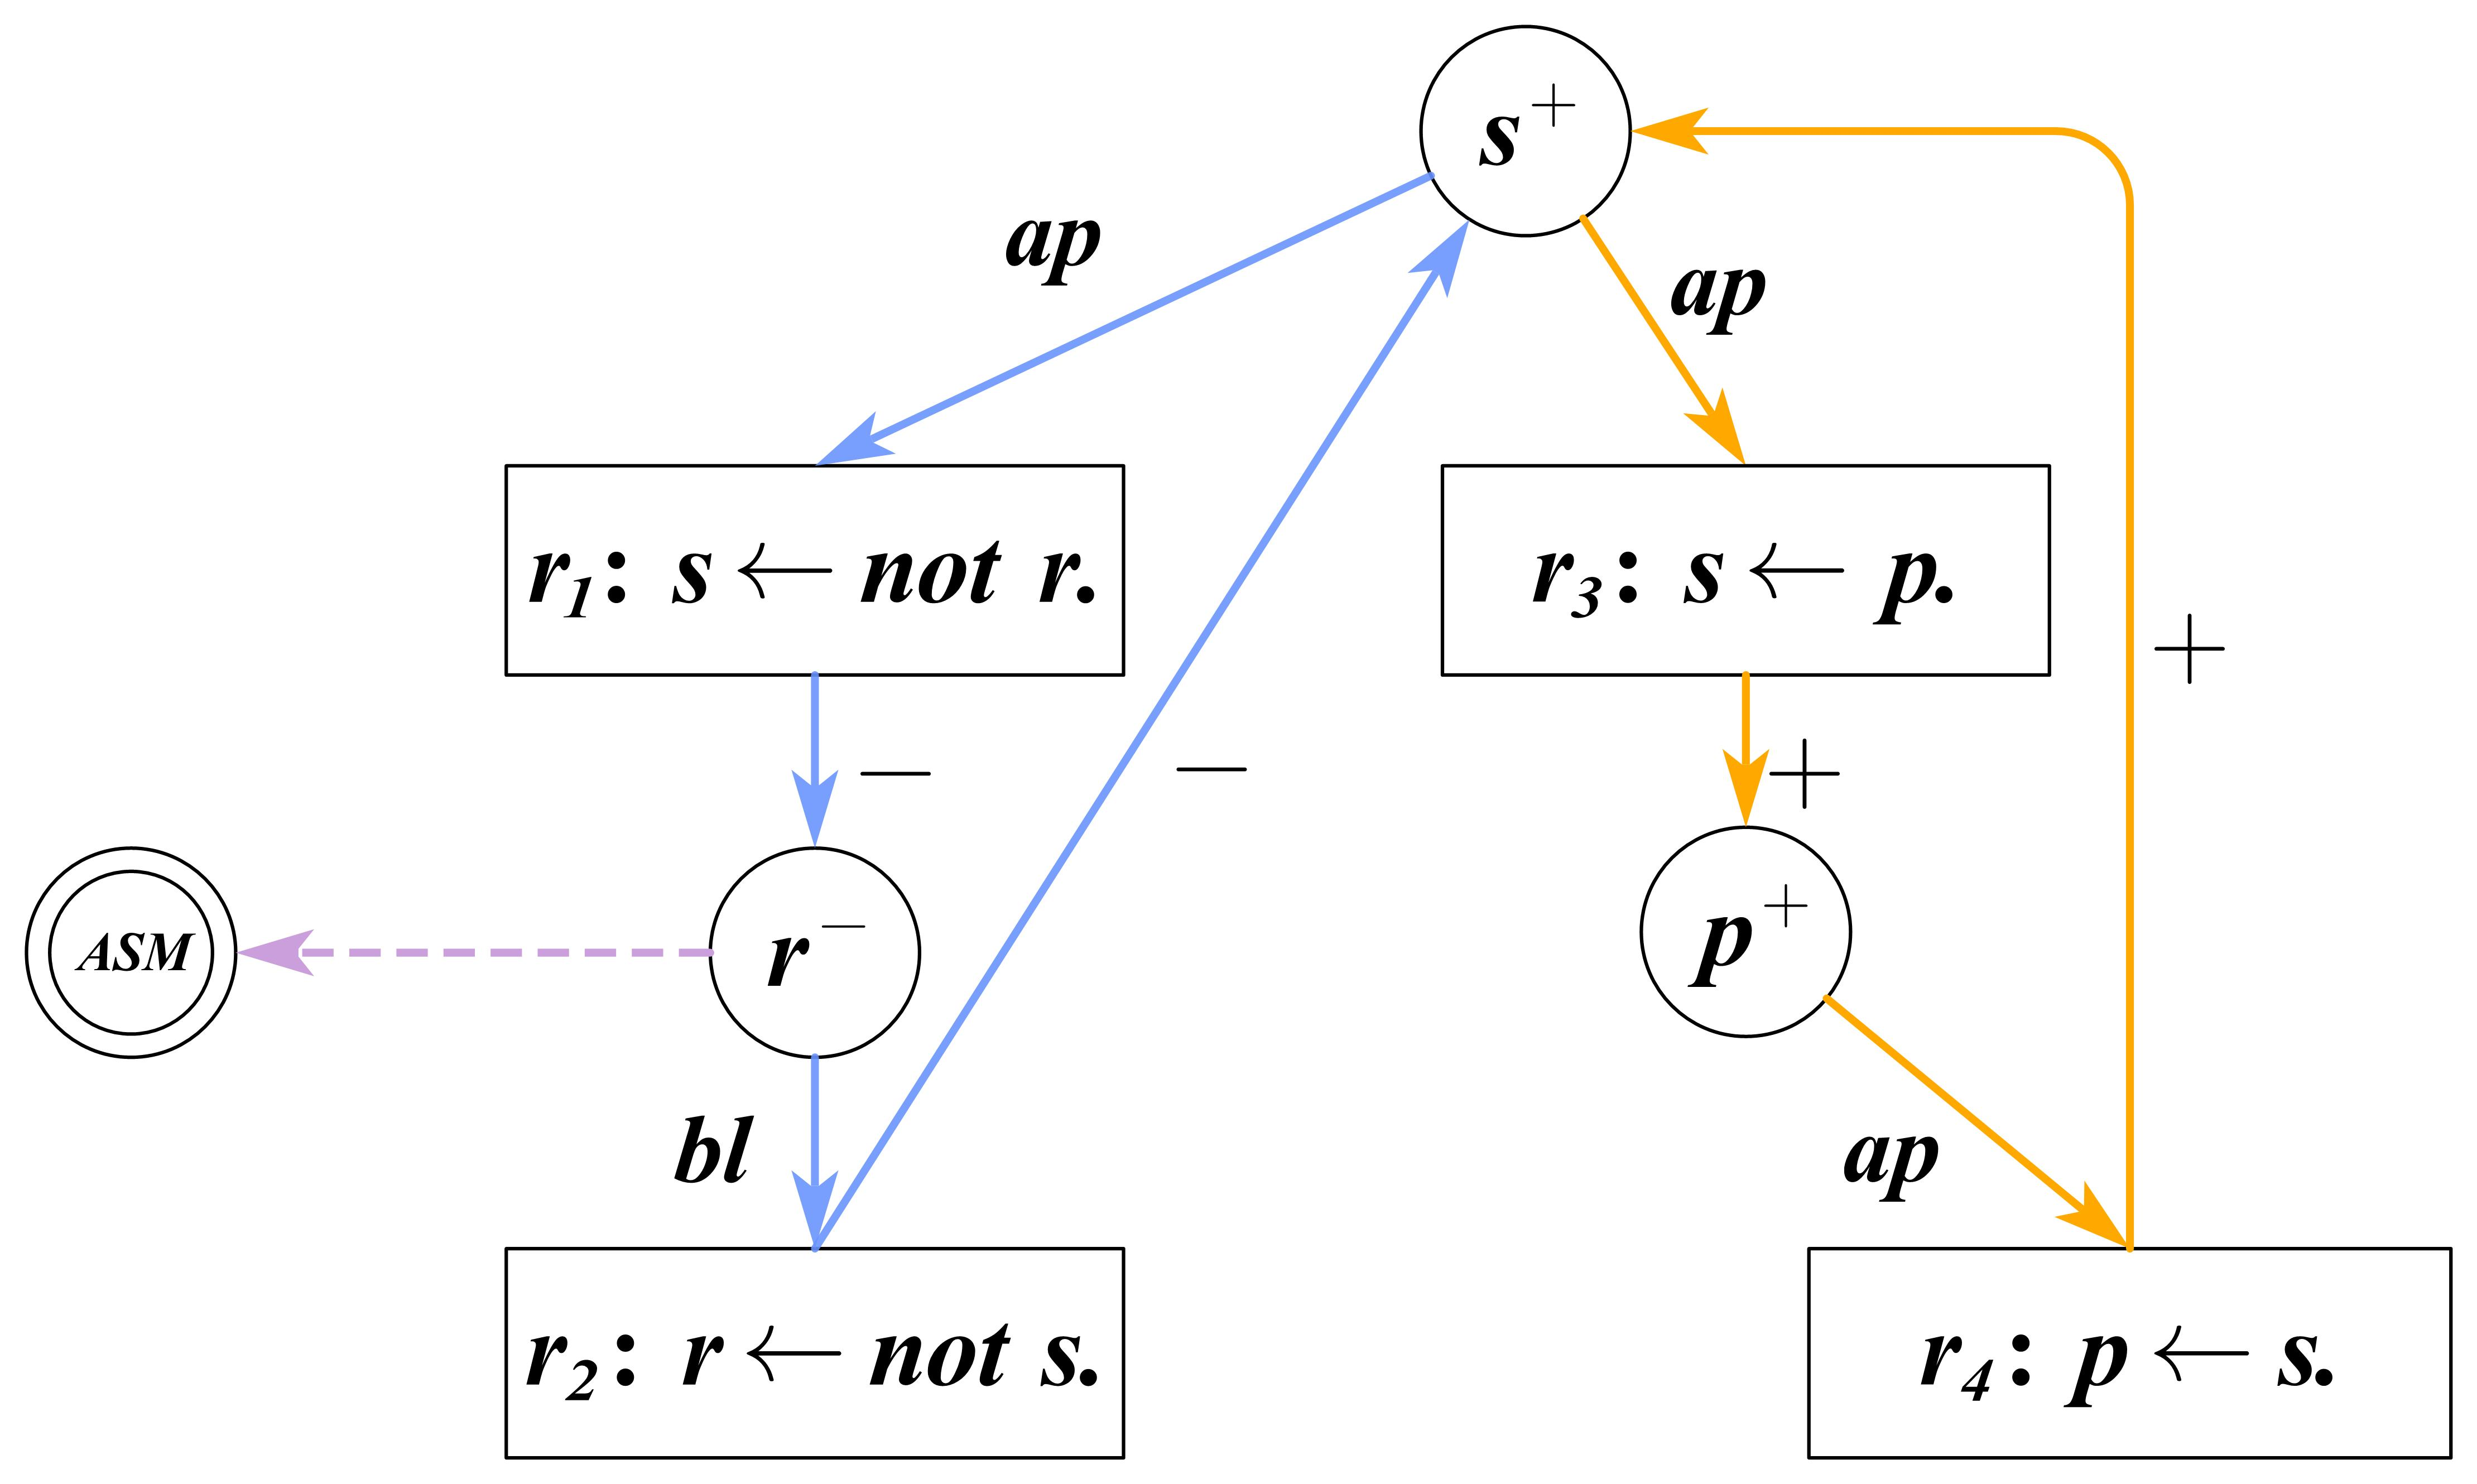
\includegraphics[height=.25\textwidth, valign=c]{figures/解释空间_2.jpg}} 
        \caption{程序\hyperref[prg:p_4]{$P_4$}在不同回答集与假设集下的两个解释空间}
        \label{fig:3_7}
    \end{figure}
    
    观察图\ref{fig:3_7}(a)可以发现,对于$s^-$而言,其真值为假既可以通过$s$位于“未受支持的正环”进行解释($UE$),也可以通过对其进行了为假的假设($ASM$)来解释。但是,通过进一步探究可以发现,正环未受支持,即规则$r_1$不适用,这一结论又需要通过$r^+$进行解释,而$r^+$再次通过规则$r_2$与$s^-$构成依赖关系。这一发现为后续构建解释时提供了一个重要的原则,即当某原子同时出现在未受支持的正环与负环中且其属于备选假设集合时,应当优先选择$ASM$进行解释。
\end{example}

\subsection{解释空间构建算法设计}
基于上述定义,下面给出解释空间生成的算法。本文的工作在花琪等人的解释空间\cite{huaqi2018lp}基础之上,重点增加了对解释空间中环处理的工作,其对应的流程如图\ref{fig:3_8}所示。
\begin{figure}[!h]
    \centering 
    \includegraphics[height=0.9\textwidth, valign=c]{figures/解释空间构建.jpg}
    \caption{程序\hyperref[prg:p_4]{$P_4$}在不同回答集与假设集下的两个解释空间}
    \label{fig:3_8}
\end{figure}

首先对ASP程序进行语法解析,构建文字结点集合$V_{atom}$、规则结点集合$V_{rule}$、汇结点集合$V_{sink}$,然后将其依赖关系通过规则适用边、原子依赖边、终结边进行连接形成图,并根据回答集对各结点与边进行正确的标记。进一步检测图中的环,若该环不存在出口,判定其为正环或负环,若为不存在出口的正环,判定其是否受到外部支持,若不受支持则将其中文字连接至$UE$结点;若为不存在出口的负环,计算可能的备选假设集,上述过程如算法\ref{alg:EU}所示。

\begin{algorithm2e}[H]
    \DontPrintSemicolon
    \SetKwInput{Initialization}{初始化}
    \SetKwInput{KwIn}{输入}
    \SetKwInput{KwOut}{输出}
    \setstretch{1.15}
    \caption{获取ASP程序$P$的解释空间}
    \label{alg:EU}
    \KwIn{一般ASP逻辑程序$P$,回答集$M \in SM(P)$}
    \KwOut{解释空间 $\mathit{EU_{P}=\langle V_{EU}, E_{EU} \rangle}$}
    \setcounter{AlgoLine}{0}
    \everypar={\nl}
    \Initialization{$V_{lit} = V_{rule} = E_{dep} = E_{end} \gets \phi$}
    \Initialization{$V_{sink} \gets \{ \text{\textit{Fact, NH, ASM, UE}}\}$}
    \ForEach{规则 $r$ 在 $P$所有规则中}{
      \If {$body(r) = \phi$}{
      $E_{end} =  E_{end} \cup (r, +, Fact)$
      }
      \If {$head(r)$不在$V_{EU}$中}{
        $V_{lit} = V_{lit} \cup head(r)$\;}
            \eIf {$M \models body(r)$}
                {$E_{ap} = E_{ap} \cup (head(r), ap, r)$\;}
            {
               $E_{ap} = E_{ap} \cup (head(r), bl, r)$ \;}
      \ForEach{文字$l$在\ $body(r)$中}{
        \If {$l \notin V_{lit}$}{
          $V_{lit} = V_{lit} \cup l$\;
        }
        \eIf {$l \in body^+(r)$}
        {$E_{dep} = E_{dep} \cup (r, +, l)$\;}
        {$E_{dep} = E_{dep} \cup (r, -, l)$\;}
      }
    }
    \ForEach {$v_{lit}$在$V_{lit}$中}{
        \If {$v_{lit}$ 出度为0}
            {$E_{end} = E_{end} \cup (v_{lit}, -, NH)$\;}
    }
    $cycles=$getAllCycles($V_{EU}$) // 找到当前图中的所有环集合cycles 
    \ForEach {$cycle$在所有环集合$cycles$中}{
    \If {$cycle$没有出口且为不被支持的正环}{
        \ForEach {$v_{lit}$在$cycle$中}
            {$E_{end} = E_{end} \cup (v_{lit}, -, UE)$}
    }
    \If {$cycle$没有出口且为不被支持的负环}
        {通过公式$\eqref{eq:asm}$计算$ASM$,由用户选择$U \in ASM$作为假设\;
        \ForEach {$v_{lit}$ in $U$}
           {$E_{end} \cup (v_{lit}, -, ASM)$}
        }
    }

    $V_{EU}=V_{lit} \cup V_{rule} \cup V_{sink}, E_{EU}= E_{dep} \cup E_{end}$\\
    \textbf{return} $\langle V_{EU}, E_{EU} \rangle$ 
\end{algorithm2e}


\section{ASP程序交互解释模型设计}
在定义了解释空间后,本文介绍对ASP程序交互解释模型的设计。下面首先通过给出该模型的输入与输出,定义可交互解释模型。
\begin{definition}[可交互解释模型]
    给定一个实例化、一致性ASP程序$P$及$P$的一个回答集$M$,$P$的解释模型$Exp_{cst}(P, s, INT(s))$有三个参数作为输入:
    \begin{itemize}[topsep=0pt]
        \setlength\itemsep{-0.3em}
        \item 实例化、一致性ASP程序$P$
        \item 当前解释步$s$,$s$是自然数
        \item 第$s$步的交互式信息$INT(s)$,这些信息包括:
        \begin{itemize}[label=$\circ$,topsep=0pt]
            \setlength\itemsep{-0.3em}
            \item 用户选择的稳定模型$M_s$,$M \in SM(P)$
            \item 用户当前步骤需要获取的解释$At_{exp_{s}}$,$At_{exp_{s}} \in Atom(P)$
            \item 用户选择的假设为假的集合$U_s$,$U_s \in Assumption(P, M)$
            \item 用户当前步骤选择展示的结点$v_s$,$v_s \in EU^{M, U}_P$
            \item 用户的当前步骤的退出信号$Q_s$,$Q_s \in \{true, false\}$
        \end{itemize}
    \end{itemize}
    
    上述符号中的下标$s$用于区分用户在不同交互步骤$s$下所提供的交互信息,这些交互信息满足如下约束:
    \begin{enumerate}[label=(\arabic*),topsep=0pt]
        \setlength\itemsep{-0.3em}
        \item $\forall i \ge 0, M_i = M_0, U_i=U_0, At_{exp_i}=At_{exp_0}$;
        \item $v_s \in \{v \mid v_{s'} \text{ 在第 }\ s' < s\ \text{ 步已经被选中,且边 }\ (v_{s'}, \cdot, v)\ \text{在}\ EU^{M, U_s}_P\ \text{中存在}\}$
    \end{enumerate}
    
    上述约束(1)表示在一次调试会话中,回答集、待解释原子和假设为假的集合被选定后,后续过程中将不再变化;约束(2)限制每一步能够被选择的结点只能是解释空间中与当前已展示出的结点一步可达的结点。

    该模型的输出$Exp_{cst}(P, s, INT(s))$如式\eqref{eq:expcst}所示:
    \begin{align}
        \label{eq:expcst}
        Exp_{cst}(P, s, INT(s))=
        \begin{cases}
        At_{exp_0} &s = 1, Q_s = false\\
        Exp_{cst}(P, s-1, INT(s-1)) &s > 1, Q_s = true\\
        Exp_{cst}(P, s-1, INT(s-1)) \cup v_s \cup Edge(v_s) & s > 1, Q_s = false\\
        \emptyset &\text{否则}\\
      \end{cases}
    \end{align}
    
    其中,$Edge(v_s)=\{(v_T, \cdotp, v_s) \mid v_T \in Exp_{cst}(P, s-1, INT(s-1)), (v_T, \cdotp, v_s) \in EU_{P}^{M,U}\}$
\end{definition}

由公式\eqref{eq:expcst}可以看出,该模型引入了解释步的概念,每一步都接受用户的一种选择,并指定用户当前关注的规则或文字。如果用户在当前步骤发送退出信号,或者如果没有其他有效节点可供用户选择,则该解释过程终止。实际上,交互式解释模型在任何步骤的输出都是解释空间的子图,并且解释构造的过程可以视为子图匹配。在这一过程中,对用户的引导和交互策略的设计至关重要。

接下来,本文具体讨论模型中的交互。模型中的交互的触发条件主要包括如下几个方面:
\begin{itemize}[topsep = 0pt]
    \item 解释开始前:
        \begin{enumerate}[label=(\arabic*), topsep = 0pt]
            \setlength\itemsep{-0.3em}
            \item 用户从多个回答集中选择指定的回答集;
            \item 用户从备选假设集合中选择指定的假设为假的原子集;
        \end{enumerate}
    \item 解释进行中:
       \begin{enumerate}[label=(\arabic*), topsep = 0pt]
            \setlength\itemsep{-0.3em}
            \item 当某条规则体部不唯一时,用户选择不同文字结点;
            \item 当某个文字位于多条规则头部时,用户选择不同的规则结点;
        \end{enumerate}
    \item 解释结束后:
        \begin{enumerate}[label=(\arabic*), topsep = 0pt]
            \setlength\itemsep{-0.3em}
            \item 用户对解释图进行存储和读取;
            \item 用户对得到的解释图进一步优化,仅查看适用的规则/阻塞的规则/最直接的文字依赖。
        \end{enumerate}
\end{itemize}

尽管用户可以在每一步骤下选择任何满足上述约束的节点,作为辅助工具,模型仍然希望通过引导与提示使得用户更便利地获取到交互解释。首先,由前面的定义和分析可以发现,假设集的概念对于用户而言并不直观。这一集合在图中体现为没有出口的负环,相较之下以图的形式对环进行展示,能够更直观准确地引导用户做出选择。另一方面,根据3.3.1中的分析可以知道,当某文字同时出现在未受支持的正环与负环中且其属于备选假设集合时,应当提示用户优先选择假设集作为解释。最后,从获取最直接解释的角度看,对于能够一步到达汇结点的文字,应当优先推荐用户查看与汇结点相连的解释。

\section{非实例化程序的变量处理}
上述对于ASP程序的解释的讨论,均面向实例化的ASP程序。但在实际应用中,程序中的变量是不可忽略的。本节讨论对非实例化程序中变量处理的方法,重点说明当前实例化工具面向解释的局限,同时给出解决这一局限性的方案。

\subsection{实例化工具\textsf{GRINGO}在ASP程序解释中的存在的问题}
为了获得一个实例化的程序,可以考虑直接采用现有的实例化工具(如\textsf{GRINGO}\cite{gebserGringoNewGrounder2007})。这些工具经过了多轮的版本迭代,不断优化\cite{gebser2011advances,gebser2015abstract},已经被稳定高效地应用于ASP程序的实例化问题中\cite{kaufmannGroundingSolvingAnswer2016}。

然而,在\textsf{GRINGO}的优化过程是面向求解的。通过\textsf{GRINGO}进行实例化得到的程序将会在保证回答集一致的情况下,被简化与改写。具体地,\textsf{GRINGO}对程序进行的简化包括:

\begin{itemize}[topsep = 0pt]
    \setlength\itemsep{-0.3em}
    \item 删除程序中体部不能被事实所满足的规则;
    \item 删除程序规则体部中能被事实满足的部分
\end{itemize}

\begin{example}[\textsf{GRINGO}的优化]
    考虑下面的非实例化程序$P_6$:
    \begin{align*}
        &r_1: fly(X) \leftarrow bird(X), not\ neg\_fly(X). \\
        &r_2: neg\_fly(X) \leftarrow penguin(X).\\
        &r_3: bird(tux).\\
        &r_4: bird(tweety).\\
        &r_5: penguin(tweety).
    \end{align*}
\end{example}

\begin{table}[!ht]
    \caption{程序$P_6$的预期实例化结果与在\textsf{GRINGO}实例化器下的实例化结果}
    \label{tb:3-1}
    \renewcommand{\arraystretch}{1.5}
    \begin{tabular}{ll}
    \hline
    期待的实例化结果$grd_{expect}(P_6)$ & \textsf{GRINGO}的实际输出$grd_{gringo}(P_6)$\tablefootnote{此处的执行的命令为: \texttt{gringo p\_6.lp -t --keep-fact}} \\ \hline
    \adjustbox{valign=t}{\begin{tabular}[c]{@{}l@{}}
        $fly(tux) \leftarrow bird(tux),$
        $\dashedbox{not\ neg\_fly(tux).}$\\ 
        $neg\_fly(tweety) \leftarrow penguin(tweety).$\\ 
        $\dashedbox{fly(tweety) \leftarrow bird(tweety), not\ neg\_fly(tweety).}$\\
        $\dashedbox{neg\_fly(tux) \leftarrow penguin(tux).}$
        \end{tabular} }
    &\adjustbox{valign=t}{ 
    \begin{tabular}[c]{@{}l@{}}
        $fly(tux) \leftarrow bird(tux).$\\
        $neg\_fly(tweety) \leftarrow penguin(tweety).$
    \end{tabular}
     } \\ \hline
    \end{tabular}
\end{table}

    该程序的唯一回答集为$M=\{bird(tux), bird(tweety), penguin(tweety),neg\_fly(twee\\\text{-}ty),fly(tux)\}$。从表\ref{tb:3-1}可以看出,由\textsf{GRINGO}得到的实例化程序与预期的实例化程序相比,第一条规则的负体部$not\ neg\_fly(tux)$被删除,三四两条规则整体没有出现在$grd_{gringo}(P_6)$中。为了更直观地说明这样的实例化为解释带来的困难,下面给出这两种实例化程序(在$M$下)对应的解释空间,如图\ref{fig:3_9}(a)与(b)所示。

    \begin{figure}[htbp] 
        \centering 
        \subfloat[$grd_{expect}(P_6)$在$M$下的解释空间]{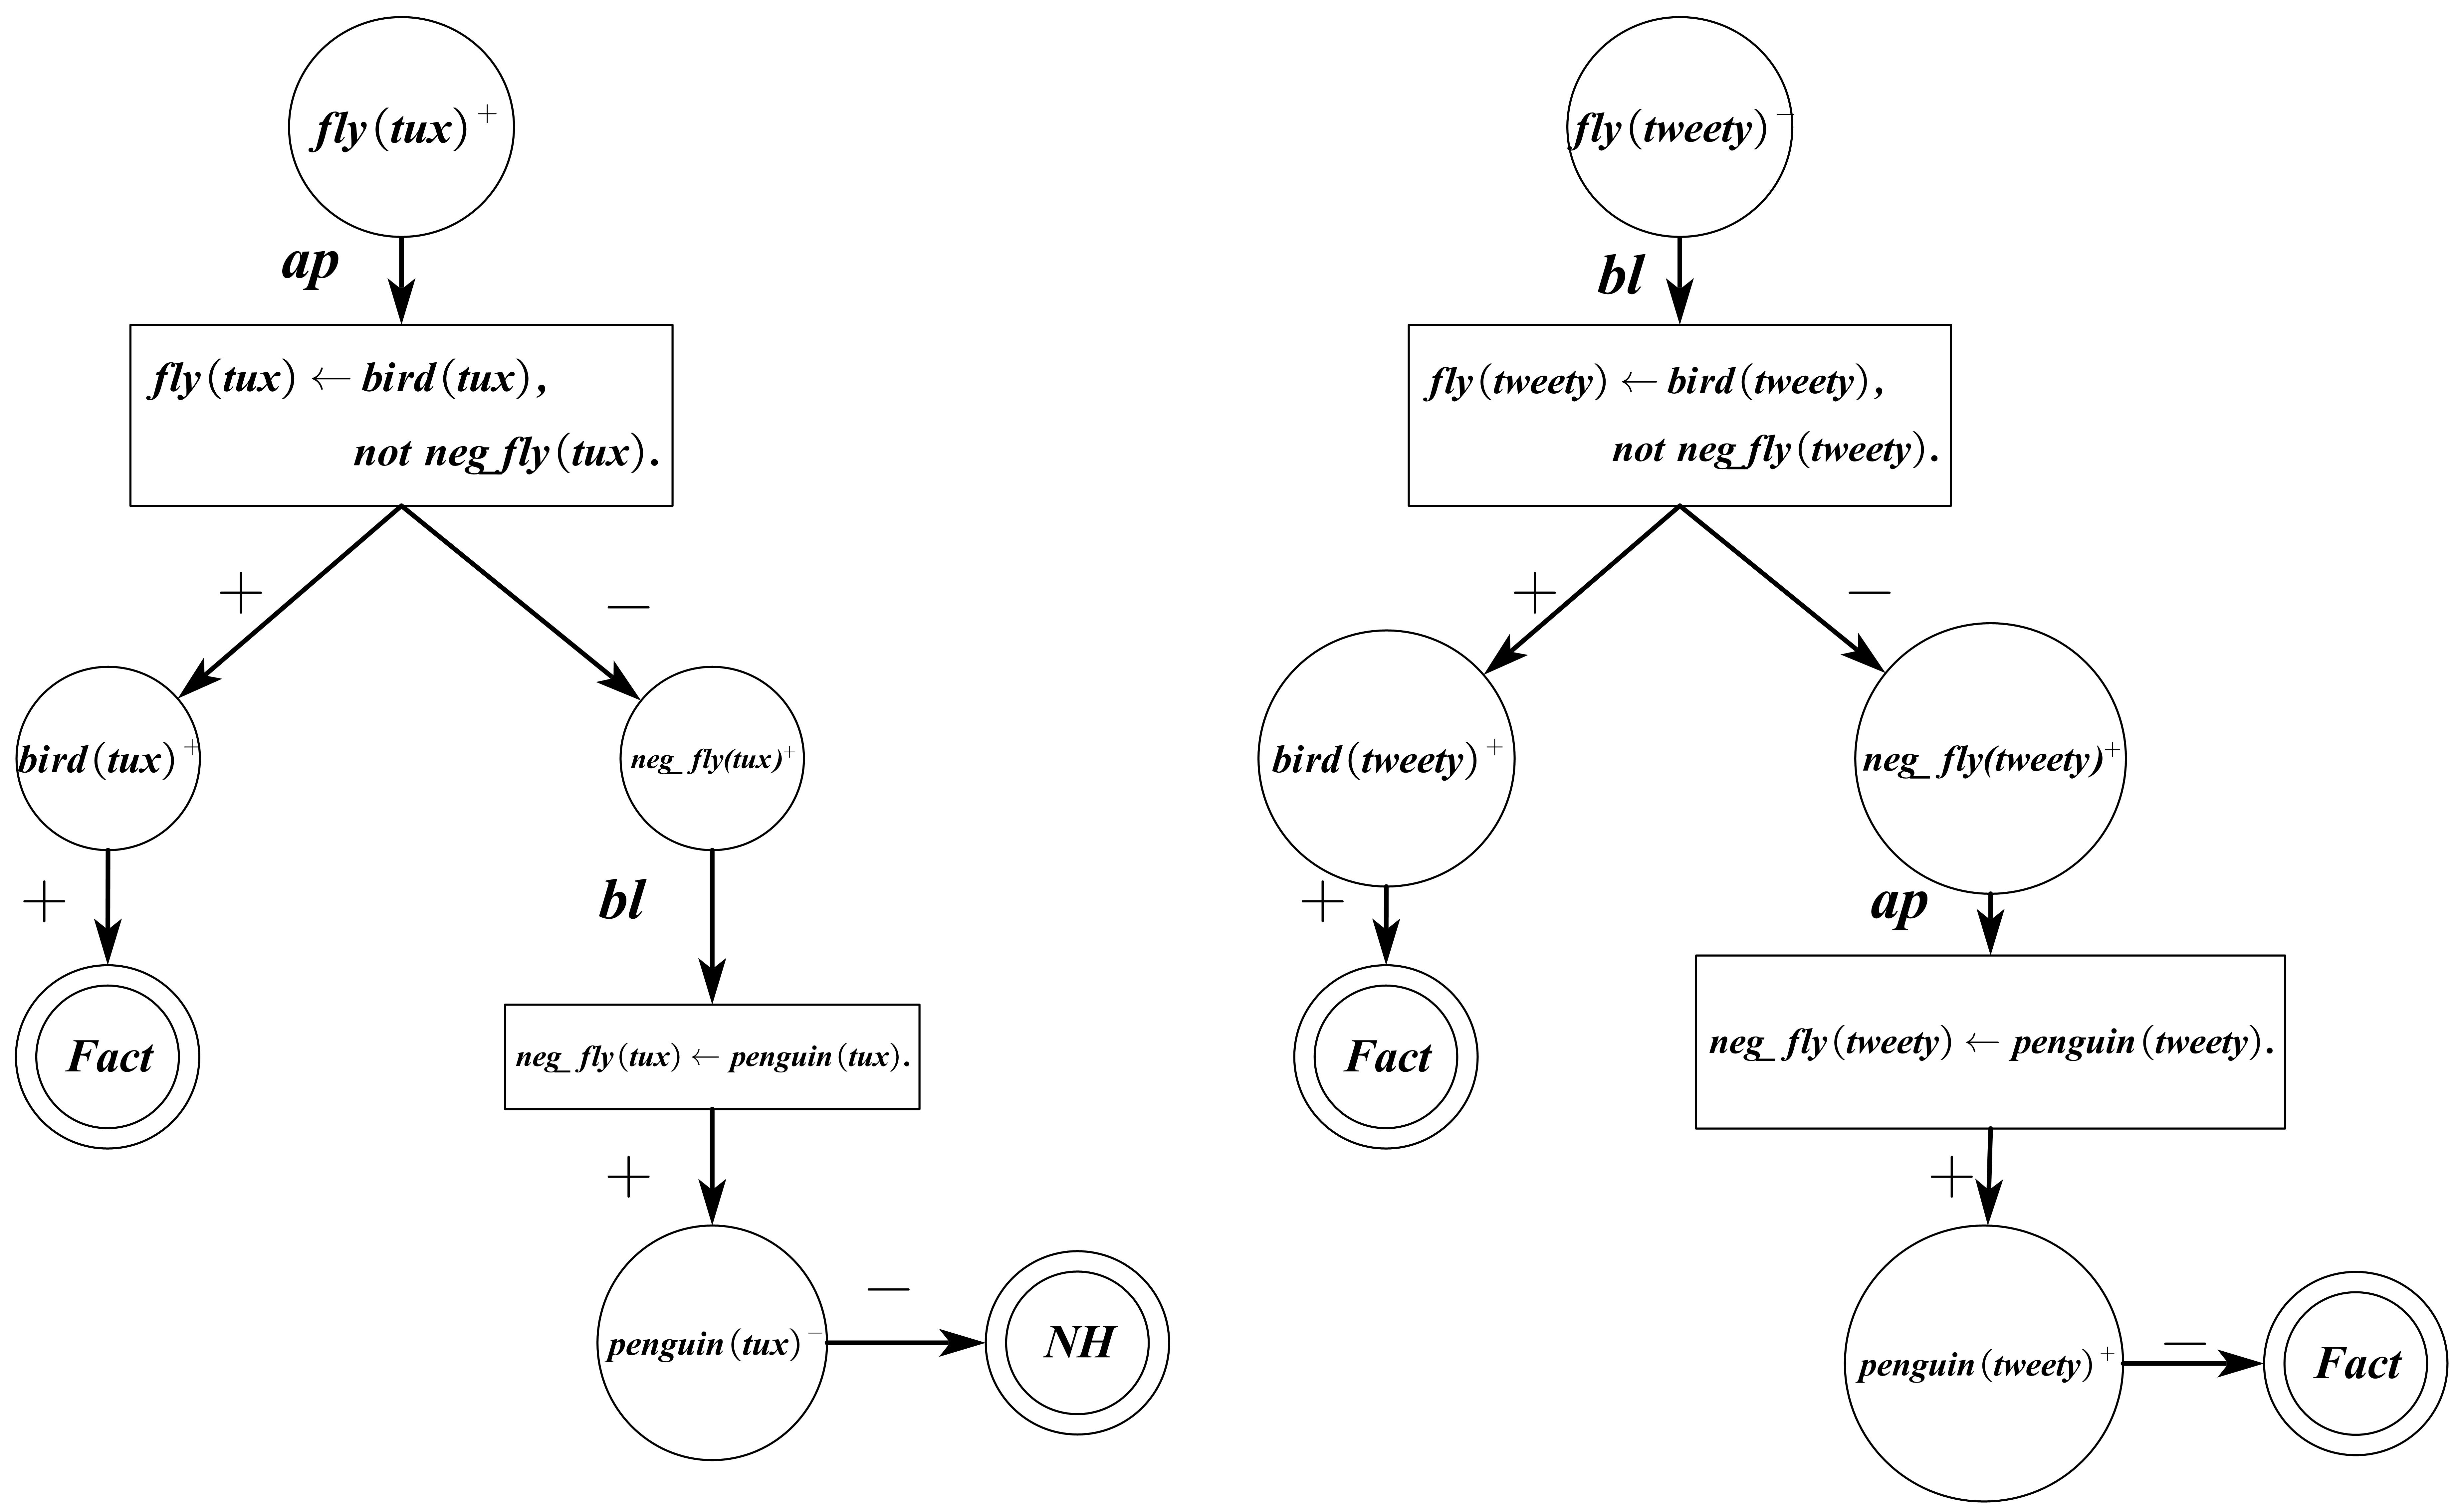
\includegraphics[height=.6\linewidth]{figures/p6解释空间-expect.jpg}} 
        \quad\quad
        \subfloat[$grd_{gringo}(P_6)$在$M$下的解释空间]{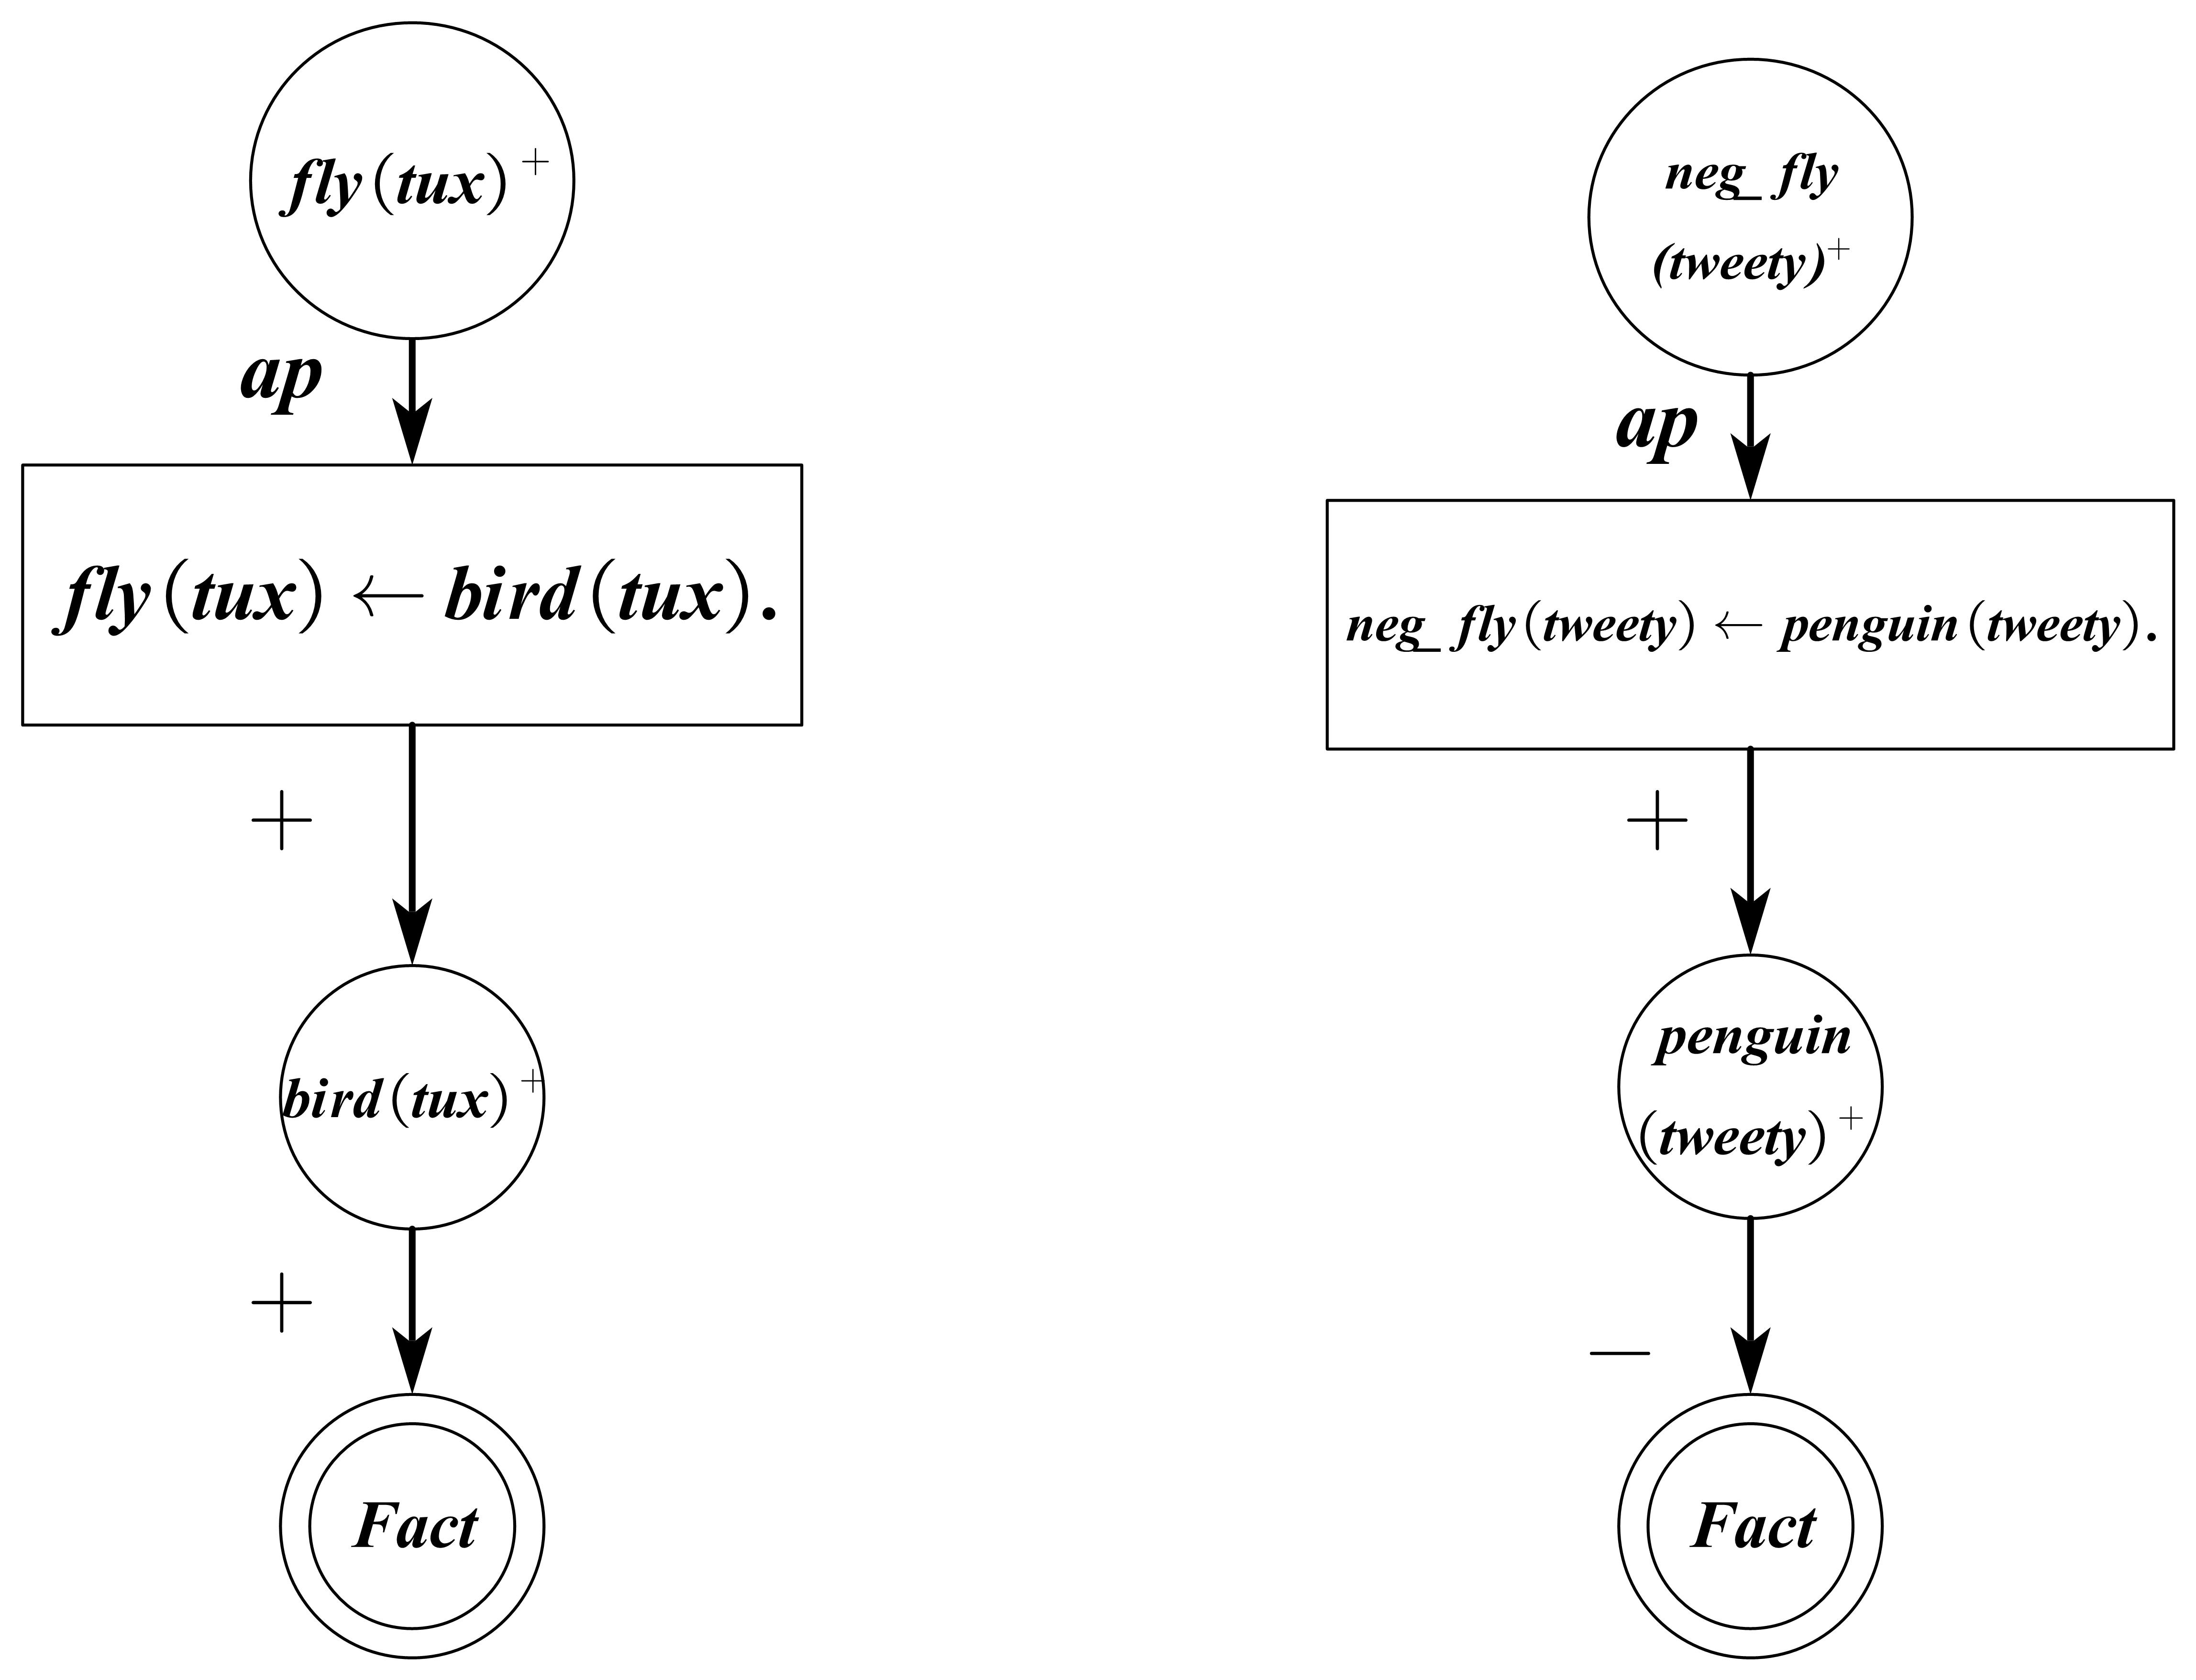
\includegraphics[height=.6\linewidth]{figures/p6解释空间-gringo.jpg}} 
        \caption{程序的两种图表示方法示意} 
        \label{fig:3_9} 
    \end{figure}

    很显然,当要求解释“\textbf{为什么tux能飞}”时,由\textsf{GRINGO}得到的实例化程序所构建的解释空间中,仅能解释为“\textbf{因为tux是鸟}”。而程序$P_6$的重点就是在于进行关于“\textbf{鸟类中不能飞的特例}”的推理,\textbf{解释tux能够飞还需要说明其不是鸟类中的特例},仅仅将“tux是鸟”作为解释显然是不够的,这一部分在$grd_{expect}(P_6)$中可以很好地得到解释;另一方面,对$tweety$来说,$grd_{gringo}(P_6)$得到的解释空间中甚至不包含$fly(tweety)$这一结点,更无从谈及对其进行解释。本文提出的解释,要求既能够对文字在回答集中的原因进行解释,也能够对不成立的文字进行解释。综上所述,由\textsf{GRINGO}得到实例化程序不能够满足本文对于解释的需求。

\subsection{基于元编程的交互式实例化方案}
    上文已经说明,\textsf{GRINGO}的版本迭代与优化已经使其具有高性能的实例化能力,因此本文仍然采用该工具进行实例化。在明确了部分规则与规则中的文字被简化或删除的原因后,通过元编程的方式,枚举每条规则体部的可满足性情况,通过编写一个上层的ASP程序,在对应的回答集中找出完整的实例化结果。为了实现对于程序的转换,参考Brain等人在\textsf{SPOCK}中的Kernel Transformation,下面给出定义程序$P$的核变换。

    \begin{definition}[程序$P$的核变换$\mathcal{K}$]
        给定一个非实例化的ASP程序$P$,$r$是$P$中的一条非事实规则($body^+(r) \cup body^-(r) \neq \emptyset$):
        \begin{align}
            \mathbf{head(r)} \leftarrow \mathbf{  body^+(r), \text{not } body^-(r)} 
        \end{align}
        
        其中,$\mathbf{head(r), body^+(r), body^-(r)}$分别表示规则$r$的头部、正体部和负体部。该规则的核变换$\mathcal{K}(r)$定义为:
        \begin{align}
            \mathcal{K}(r)= K_{ap}(r) \cup K_{blp}(r) \cup K_{bln}(r)
        \end{align}
        其中:
        \begin{align}
            &K_{ap}(r)=ap(head(r), p(body^+(r)), n(body^-(r))) \leftarrow body^+(r), not\ body^-(r) \label{eq:kap}\\
            &K_{blp}(r)=\bigcup\limits_{{l \in body^+(r)}} \left(bl(head(r), p(body^+(r)), n(body^-(r)))\leftarrow not\ l, var(X) \right) \label{eq:blp}\\
            &K_{bln}(r)=\bigcup\limits_{{l \in body^-(r)}} \left(bl(head(r), p(body^+(r)), n(body^-(r)))\leftarrow l, var(X) \right) \label{eq:bln}
        \end{align}
        则程序$P$的核变换$\mathcal{K}(P)$定义为:
        \begin{align}
            \mathcal{K}(P) = \left( \bigcup_{\substack{r \in P,\\body^+(r) \cup body^-(r) \neq \emptyset}}\mathcal{K}(r) \right) \cup P
        \end{align}
    \end{definition}

    \begin{theorem}[程序的核变换有且仅有一个回答集]
        \label{thm:kernel}
        给定一个ASP程序$P$, 其核变换$\mathcal{K}(P)$ 有唯一回答集。
    \end{theorem}

    \begin{proof}[定理\ref{thm:kernel}的证明]
        $\forall r' \in \mathcal{K}(P), head(r') \in \{ap/3, bl/3\}$, 且 $body(r') \cap \{ap/3, bl/3\} = \phi$, 因此$\mathcal{K}(P)$不包含环。 Kunen等人提出不包含环的ASP程序称为调用一致性程序(call-consistent)\cite{kunen1989signed}。 Papadimitriou等人证明了调用一致性ASP程序有且仅有一个回答集\cite{PAPADIMITRIOU199748},因此定理\ref{thm:kernel}成立。
    \end{proof}

    式\eqref{eq:kap}-\eqref{eq:bln}是核变换的三组核心规则,这三组规则实际上枚举了一条ASP规则体部的三种满足性情况:同时满足正体部与负体部、不满足正体部、不满足负体部。在这样的情况下,无论程序中的事实如何,对事实中的每一个对象常量$c$和程序中的每一个非事实的实例化规则$r$而言,一定能找到规则$r' \in \mathcal{K}(r)$,使得$c$被实例化进入$r'$体部的项中。

    \begin{example}[程序$P_6$的核变换]
        为程序$P_6$进行核变换,得到的$\mathcal{K}(P_6)$为:
        \begin{align*}
            &fly(X) \leftarrow bird(X), not\ neg\_fly(X).\\
            &\dashedbox[colback=gray!30]{ap(head(fly(X)), p(bird(X)), n(neg\_fly(X))) \leftarrow bird(X), not\ neg\_fly(X).}\\
            &\dashedbox[colback=gray!30]{blp(head(fly(X)), p(bird(X)), n(neg\_fly(X))) \leftarrow not\ bird(X), var(X).}\\
            &\dashedbox[colback=gray!30]{bln(head(fly(X)), p(bird(X)), n(neg\_fly(X))) \leftarrow neg\_fly(X).}\\
            &neg\_fly(X) \leftarrow penguin(X).\\
            &\dashedbox[colback=gray!30]{ap(head(neg\_fly(X)), p(penguin(X)), n()) \leftarrow penguin(X).}\\
            &\dashedbox[colback=gray!30]{blp(head(neg\_fly(X)), p(penguin(X)), n()) \leftarrow not\ penguin(X), var(X).}\\
            &bird(tux;tweety).\\
            &penguin(tweety).\\
            &var(tux;tweety).
        \end{align*}
    
        $\mathcal{K}(P_6)$的回答集中关于原子ap、blp和bln的文字为:
    \begin{align*}
        \{&ap(head(neg\_fly(tweety)),p(penguin(tweety)),n),\\
        &ap(head(fly(tux)),p(bird(tux)),n(neg\_fly(tux))),\\
        &bln(head(fly(tweety)),p(bird(tweety)),n(neg\_fly(tweety))),\\
        &blp(head(neg\_fly(tux)),p(penguin(tux)),n)\}
    \end{align*}
    
    逐条对上述文字中的head项、p项和n项中的项进行提取,可以得到对应的完整实例化程序:
    \begin{align*}
        &neg\_fly(tweety) \leftarrow penguin(tweety).\\
        &fly(tux) \leftarrow bird(tux), neg\_fly(tux).\\
        &fly(tweety) \leftarrow bird(tweety), neg\_fly(tweety).\\
        &neg\_fly(tux) \leftarrow penguin(tux).
    \end{align*}
    \end{example}

    然而,上述方案在实现过程中可能出现空间复杂度过大的问题。对于一个有$n$个变量的ASP程序,假设不同的对象常量数量为$c$,那么所有不同的实例化替换的方式理论上有$n^c$个,而实际上有些实例化在应用中是冗余的。考虑程序$P_6 \cup \{cat(elvis).\}$。此时,$elvis$作为猫的名字,与整个程序$P_6$所讨论的物种不再相关,因此将其放入实例化程序中似乎没有必要。但是,用户依然有可能寻求解释:\textbf{为什么elvis不会飞?}。此时,仍需要借助规则$fly(elvis) \leftarrow bird(elvis), neg\_fly(elvis).$来进行解释。因此,考虑通过在实例化前进行用户交互,进一步缩减实例化规模。注意到上文中,增加了一个辅助文字$var$,这一文字用于保证Clingo语法下规则的安全性(Safety)。具体来说,所谓安全的规则,是指出现在规则负体部的文字必须至少在头部或正体部内也出现一次\cite{calimeri2020aspcore2}。而在核变换中对正体部错误情况进行枚举时,将会出现规则仅有一个负体部的情况。此时,若用户能够指定一个“最基础的谓词”,满足“违背该谓词的情况不予考虑”,则能够降低程序的规模。例如,若用户指定违背$bird(X)$的情形不予考虑,那么上述程序中$not\ bird(X)$的规则阻塞情况将不会被枚举。另一方面,在Yuanlin Zhang等人提出的基于ASP的扩展语言\textsf{onlineSPARC},面向ASP程序的教学,通过引入了sort的概念,在程序编写时为每个变量都明确指定了最基本的域\cite{marcopoulos2019onlinesparc, balai2013answer}。本文借鉴这一工作的思路,若用户指定了最基础谓词,则继续考虑将其他谓词与之绑定。例如$neg\_fly(X)$中的$X$一定也满足$bird(X)$,以避免出现将elvis(猫名)带入关于鸟的规则中进行讨论的冗余情况出现。


    \section{本章小结}
    为了给出一个用户可接受且清晰完整的ASP回答集文字的解释,本章提出了一个基于用户交互的ASP程序解释模型并给出其构建算法。为了构建这一模型,首先对已有工作进行改进,找到了一种合适的ASP程序图表示方法——扩展原子-规则图,然后重点对图中的环进行处理,以得到ASP程序的解释空间并给出其构建算法;进一步,基于解释空间形式化定义交互解释模型并探究用户交互解释的过程,最后针对非实例化程序,研究当前实例化工具在进行解释任务中存在的局限性,通过元编程的方法给出面向解释的ASP程序实例化方案。